%%%%%%%%%%%%%%%%%%%%%%%%%%%%%%%%%%%%%%%%%%%%%%%%%%%%%%%%%%%%%%%%%%%%%%%%%%%%%%%%
%
% Template license:
% CC BY-NC-SA 3.0 (http://creativecommons.org/licenses/by-nc-sa/3.0/)
%
%%%%%%%%%%%%%%%%%%%%%%%%%%%%%%%%%%%%%%%%%%%%%%%%%%%%%%%%%%%%%%%%%%%%%%%%%%%%%%%%

%----------------------------------------------------------------------------------------
%	PACKAGES AND OTHER DOCUMENT CONFIGURATIONS
%----------------------------------------------------------------------------------------

\documentclass[
11pt, % The default document font size, options: 10pt, 11pt, 12pt
%oneside, % Two side (alternating margins) for binding by default, uncomment to switch to one side
%chapterinoneline,% Have the chapter title next to the number in one single line
spanish,
singlespacing, % Single line spacing, alternatives: onehalfspacing or doublespacing
%draft, % Uncomment to enable draft mode (no pictures, no links, overfull hboxes indicated)
%nolistspacing, % If the document is onehalfspacing or doublespacing, uncomment this to set spacing in lists to single
%liststotoc, % Uncomment to add the list of figures/tables/etc to the table of contents
%toctotoc, % Uncomment to add the main table of contents to the table of contents
parskip, % Uncomment to add space between paragraphs
%codirector, % Uncomment to add a codirector to the title page
headsepline, % Uncomment to get a line under the header
]{MastersDoctoralThesis} % The class file specifying the document structure



%----------------------------------------------------------------------------------------
%	INFORMACIÓN DE LA MEMORIA
%----------------------------------------------------------------------------------------

\thesistitle{Sistema de monitoreo de cultivos agrícolas} % El títulos de la memoria, se usa en la carátula y se puede usar el cualquier lugar del documento con el comando \ttitle

% Nombre del posgrado, se usa en la carátula y se puede usar el cualquier lugar del documento con el comando \degreename
\posgrado{Carrera de Especialización en Sistemas Embebidos} 
%\posgrado{Carrera de Especialización en Internet de las Cosas} 
%\posgrado{Carrera de Especialización en Intelegencia Artificial}
%\posgrado{Maestría en Sistemas Embebidos} 
%\posgrado{Maestría en Internet de las cosas}

\author{Ing. Mario Fernando Aguilar Montoya} % Tu nombre, se usa en la carátula y se puede usar el cualquier lugar del documento con el comando \authorname

\director{Esp. Ing. Julian Bustamante Narvaez  (TECREA SAS)} % El nombre del director, se usa en la carátula y se puede usar el cualquier lugar del documento con el comando \dirname
\codirector{Nombre del codirector (pertenencia)} % El nombre del codirector si lo hubiera, se usa en la carátula y se puede usar el cualquier lugar del documento con el comando \codirname.  Para activar este campo se debe descomentar la opción "codirector" en el comando \documentclass, línea 23.

\juradoUNO{Dr. Ing. Javier Andrés Redolfi (UTN-FRSF)} % Nombre y pertenencia del un jurado se usa en la carátula y se puede usar el cualquier lugar del documento con el comando \jur1name
\juradoDOS{Mg. Lic. Leopoldo Zimperz (FIUBA)} % Nombre y pertenencia del un jurado se usa en la carátula y se puede usar el cualquier lugar del documento con el comando \jur2name
\juradoTRES{Esp. Ing. Felipe Calcavecchia (FIUBA)} % Nombre y pertenencia del un jurado se usa en la carátula y se puede usar el cualquier lugar del documento con el comando \jur3name

%\ciudad{Ciudad Autónoma de Buenos Aires}
\ciudad{ciudad de Tarija}

\fechaINICIO{junio de 2022}
\fechaFINAL{agosto de 2023}


\keywords{Sistemas embebidos, FIUBA} % Keywords for your thesis, print it elsewhere with \keywordnames


\begin{document}


\frontmatter % Use roman page numbering style (i, ii, iii, iv...) for the pre-content pages

\pagestyle{plain} % Default to the plain heading style until the thesis style is called for the body content


%----------------------------------------------------------------------------------------
%	RESUMEN - ABSTRACT 
%----------------------------------------------------------------------------------------

\begin{abstract}
\addchaptertocentry{\abstractname} % Add the abstract to the table of contents
%
%The Thesis Abstract is written here (and usually kept to just this page). The page is kept centered vertically so can expand into the blank space above the title too\ldots
\centering
En la presente memoria se aborda el diseño e implementación de un sistema de adquisición de datos para el monitoreo de cultivos agrícolas realizado como emprendimiento personal. Este trabajo pretende ayudar al agricultor a gestionar de mejor manera sus recursos.
Para su desarrollo fueron fundamentales los conocimientos adquiridos en la carrera tales como conceptos de modularización, testing de software, sistemas operativos en tiempo real, protocolos de comunicación y programación de microcontroladores.
\end{abstract}

%----------------------------------------------------------------------------------------
%	CONTENIDO DE LA MEMORIA  - AGRADECIMIENTOS
%----------------------------------------------------------------------------------------

\begin{acknowledgements}
%\addchaptertocentry{\acknowledgementname} % Descomentando esta línea se puede agregar los agradecimientos al índice
\vspace{1.5cm}
En primer lugar a mi familia y amigos que siempre me brindan su apoyo y confianza.
\\A mi director por su paciencia, guía y consejo en todo momento.
\\A mis compañeros y maestros de la CESE, por los aportes y enseñanzas que me dieron a los largo de la especialización.



\end{acknowledgements}

%----------------------------------------------------------------------------------------
%	LISTA DE CONTENIDOS/FIGURAS/TABLAS
%----------------------------------------------------------------------------------------

\tableofcontents % Prints the main table of contents

\listoffigures % Prints the list of figures

\listoftables % Prints the list of tables


%----------------------------------------------------------------------------------------
%	CONTENIDO DE LA MEMORIA  - DEDICATORIA
%----------------------------------------------------------------------------------------

%\dedicatory{\textbf{Dedicado a... [OPCIONAL]}}  % escribir acá si se desea una dedicatoria

%----------------------------------------------------------------------------------------
%	CONTENIDO DE LA MEMORIA  - CAPÍTULOS
%----------------------------------------------------------------------------------------

\mainmatter % Begin numeric (1,2,3...) page numbering

\pagestyle{thesis} % Return the page headers back to the "thesis" style

% Incluir los capítulos como archivos separados desde la carpeta Chapters

% Chapter 1

\chapter{Introducción general} % Main chapter title
En este capítulo se hace una breve introducción a la necesidad que condujo al desarrollo del trabajo. Se presenta el internet de las cosas y el estado del arte de dispositivos similares. Asimismo, se explica el objetivo y los alcances del trabajo.
\label{Chapter1} % For referencing the chapter elsewhere, use \ref{Chapter1} 
\label{IntroGeneral}

%----------------------------------------------------------------------------------------

% Define some commands to keep the formatting separated from the content 
\newcommand{\keyword}[1]{\textbf{#1}}
\newcommand{\tabhead}[1]{\textbf{#1}}
\newcommand{\code}[1]{\texttt{#1}}
\newcommand{\file}[1]{\texttt{\bfseries#1}}
\newcommand{\option}[1]{\texttt{\itshape#1}}
\newcommand{\grados}{$^{\circ}$}

%----------------------------------------------------------------------------------------

%\section{Introducción}

%----------------------------------------------------------------------------------------
\section{Introducción}
En los últimos años la agricultura ha enfrentado muchos desafíos, desde una creciente población mundial a ser alimentada, hasta requisitos de sostenibilidad y restricciones ambientales debido al cambio climático y el calentamiento global.

La agricultura es uno de los sectores que más sufre la escasez de agua que existe actualmente en el mundo, uno de los objetivos de implementar la tecnología IoT en este sector, es el de lograr una gestión eficiente y sostenible de los recursos hídricos.

Esto obliga a implementar soluciones que permitan modernizar las prácticas agrícolas. En este contexto, la Agricultura 4.0 representa la última evolución de la  agricultura de precisión. La misma se encuentra basada en el concepto de agricultura inteligente, donde convergen el uso de internet de las cosas, computación
en la nube, aprendizaje automático para el análisis de grandes volúmenes de datos, vehículos no tripulados y robótica.

\subsection{Internet de las cosas}
El concepto de internet de las cosas o IoT (del ingles Internet of Things) se refiere a la interconexión digital de dispositivos y objetos a través de una red, es decir, dispositivos como sensores y/o actuadores, equipados con una interfaz de comunicación, unidades de procesamiento y almacenamiento. Estos dispositivos tienen la capacidad de adquirir, intercambiar y transferir datos a la red mediante alguna tecnología de comunicación inalámbrica.

El IoT puede usarse a favor de la sostenibilidad, no cabe duda de que Internet es un facilitador de iniciativas sostenibles. De acuerdo con el Foro Económico Mundial la mayoría de los proyectos con internet de las cosas se centran en la eficiencia energética en las ciudades, energías sostenibles y el consumo responsable. Por ejemplo:
\begin{itemize}
  \item Eficiencia energética: en este sector se interconectan sensores, algoritmos y redes de comunicación para anticipar la demanda eléctrica y así realizar una distribución sostenible de la energía para reducir el precio del kW.
  \item Uso del Agua: esta tecnología pone en funcionamiento máquinas para recoger datos en tiempo real que permitan hacer uso eficiente del agua y reducir su consumo.
  
\end{itemize}

\subsection{Sistemas de monitoreo de cultivos agrícolas}
Los sistemas de monitoreo de cultivos agrícolas se encargan de monitorear
las distintas variables ambientales a las que están expuestos los cultivos agrícolas, los datos adquiridos ayudan a la toma de decisiones y a manejar de una manera eficiente los recursos con los que cuentan los agricultores.

Cuentan con tres partes fundamentales: 
\begin{itemize}
  \item El nodo sensor, que en sí sería la parte física o hardware, generalmente de bajo consumo.
  \item El firmware que abarca la lógica del sistema y se encarga de realizar la adquisición, procesamiento y transferencia de datos que puede o no estar sobre un sistema operativo de tiempo real.
  \item Nube o plataforma IoT, que ofrecen diferentes servicios como ser almacenamiento, procesamiento, análisis, visualización, etc. Esta parte del sistema permite al usuario del sistema poder visualizar los valores de las variables medidas y así poder tomar decisiones con respecto a las mediciones.
\end{itemize}
%----------------------------------------------------------------------------------------

\section{Estado del arte}

Durante la etapa de investigación del proyecto se realizó la búsqueda de productos comerciales en el mercado local e internacional.
Se encontraron algunos productos de similares características al que se pretende realizar, un dato interesante a resaltar todos los productos encontrados son del mercado internacional, no se encontró ningún producto o empresa que ofrezca este tipo de soluciones
en el mercado local.

A continuación se describen los productos encontrados, estas opciones varían con respecto a la tecnología que utilizan.

\subsection{Libelium}

Smart Agriculture PRO figura 1.1 es un módulo de IoT que está diseñado para realizar monitoreo de viñedos para mejorar la calidad del vino, riego selectivo en campos de golf y control de condiciones en invernaderos, entre otros.
Permite monitorear múltiples parámetros ambientales que involucran una amplia gama de aplicaciones, desde el análisis del desarrollo en crecimiento hasta la observación del clima. Para ello se ha dotado de sensores de temperatura y humedad del aire y del suelo, luminosidad, radiación solar, velocidad y dirección del viento, precipitaciones, presión atmosférica, humedad de las hojas, distancia y diámetro del fruto o tronco.
\vspace{1cm}

\begin{figure}[htbp]
	\centering
	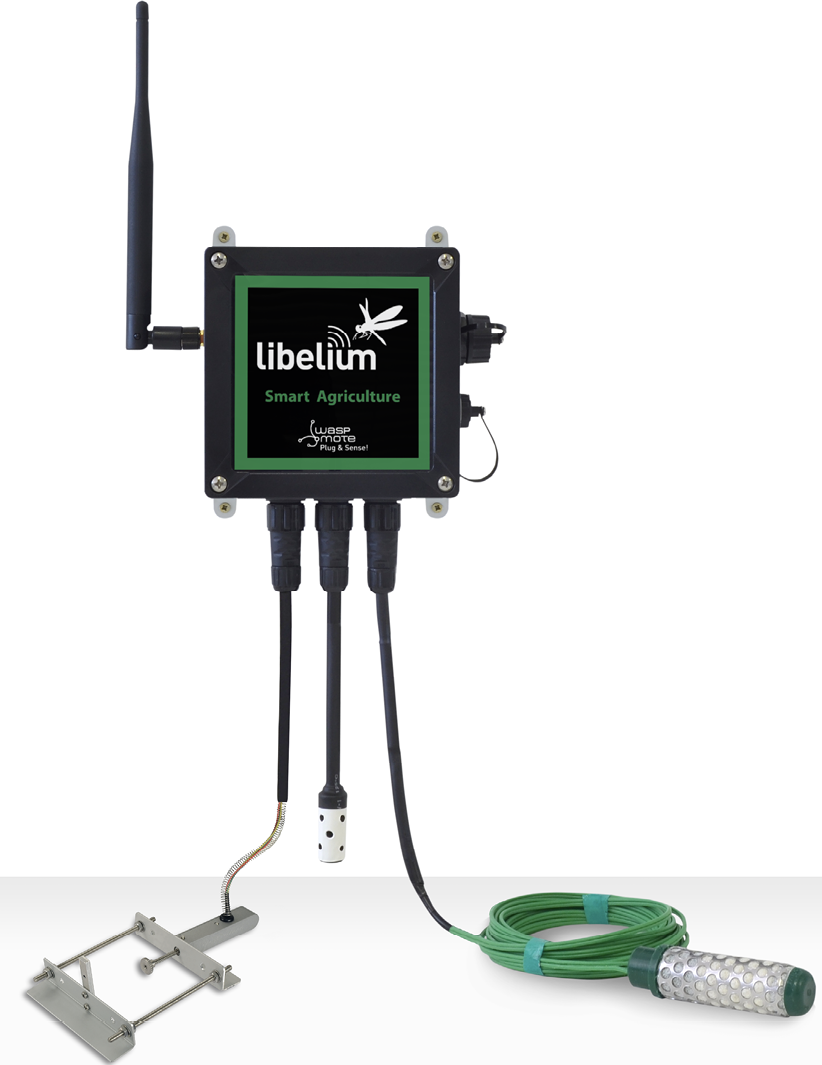
\includegraphics[width=.4\textwidth]{./Figures/modulo_libelium.png}
	\caption{Modulo Smart Agriculture PRO.}
	\label{fig:texmaker}
\end{figure}

\vspace{1cm}

\subsection{Nodo RF-M1 DropControl}

El nodo RF-M1 es adecuado para tareas de monitoreo simples como parte de una red DropControl o por sí solo. Posee una combinación de entradas que le permite realizar múltiples tareas de monitoreo y almacenarlas en la nube. En la figura 1.2 se muestra el módulo físicamente.

Características del dispositivo: 
\begin{itemize}
  \item Redes RF mesh o comunicación celular.
  \item Energía autónoma, solar + batería.
  \item Actualización del firmware vía aérea, configuraciones y soporte por internet.
  \item Protección externa IP65.
  \item Amplia variedad de compatibilidad con sensores.
  \item Unidad de bajo costo para resolver necesidades básicas de monitoreo. 
\end{itemize}

\begin{figure}[htbp]
	\centering
	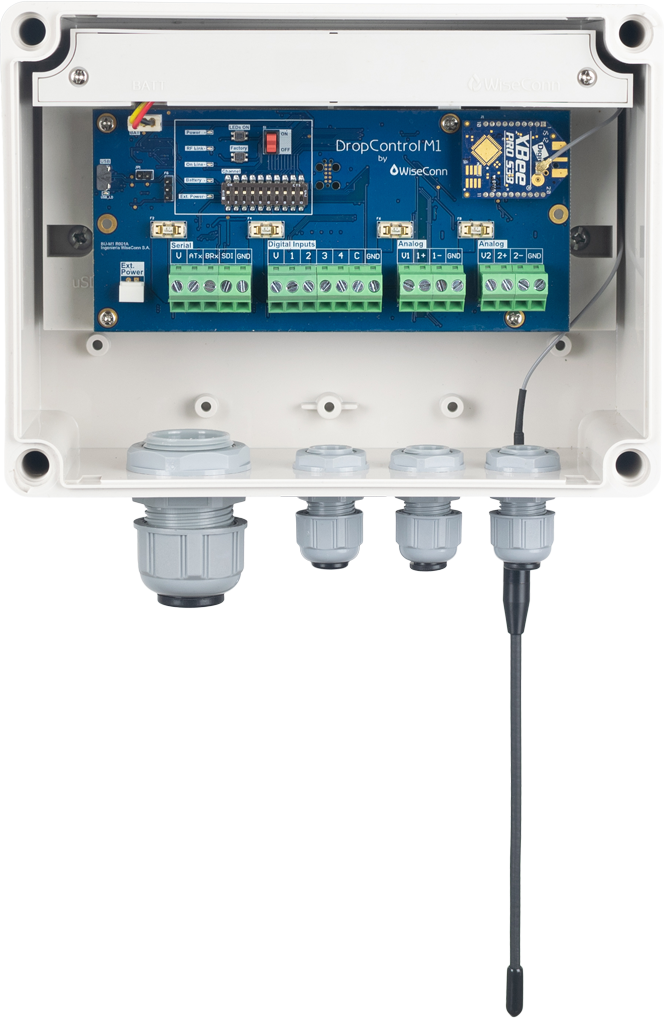
\includegraphics[width=.3\textwidth]{./Figures/modulo_dropcontrol.png}
	\caption{Modulo RF-M1 de DropControl.}
	\label{fig:texmaker}
\end{figure}

\vspace{1cm}
%----------------------------------------------------------------------------------------
\vspace{30cm}

\section{Objetivo y alcances}

\subsection{Objetivo}
El objetivo principal del trabajo es el diseño e implementación de un prototipo funcional de un sistema de monitoreo de cultivos agrícolas.
\subsection{Alcances}

\begin{itemize}
  \item Implementación de un prototipo funcional con hardware de bajo consumo. 	
  \item Desarrollo del firmware sobre un sistema operativo de tiempo real.
  \item Transmisión de la información por red celular.
  \item Visualización de los datos en Ubidots.
\end{itemize}
\chapter{Introducción específica} % Main chapter title

\label{Chapter2}

%----------------------------------------------------------------------------------------
%	SECTION 1
%----------------------------------------------------------------------------------------
Todos los capítulos deben comenzar con un breve párrafo introductorio que indique cuál es el contenido que se encontrará al leerlo.  La redacción sobre el contenido de la memoria debe hacerse en presente y todo lo referido al proyecto en pasado, siempre de modo impersonal.

\section{Componentes principales de hardware}
\label{sec:ejemplo}

\subsection{STM32 NUCLEO-L432KC}
La placa STM32 Nucleo-32 que se muestra en la figura \ref{fig:nucleol432kc} proporciona una forma asequible y flexible para que los usuarios prueben nuevos conceptos y construyan prototipos eligiendo entre las diversas combinaciones de funciones de rendimiento y consumo de energía que proporciona el microcontrolador STM32\citep{NUCLEOL432KC}.
\\Características:
\begin{itemize}
	\item Microcontrolador STM32L4KC en paquete 32 de pines.
	\item 1 led de usuario.
	\item 1 pulsador de reset.
	\item Conector de expansión Arduino Nano V3.
	\item Conector USB Micro-AB para ST-LINK.
	\item Opciones flexibles de fuente de alimentación.
	\item Depurador/Programador ST-LINK integrado.
	\item Compatibilidad con una amplia variedad de entornos de desarrollo integrado.
	\item Oscilador de cristal de 24MHz
	\item Compatible con Arm Mbed Enabled  
\end{itemize}
\begin{figure}[htbp]
	\centering
	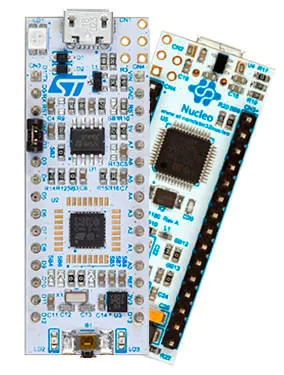
\includegraphics[width=.4\textwidth]{./Figures/nucleo-l432kc.jpg}
	\caption{Placa NUCLEO-L432KC.}
	\label{fig:nucleol432kc}
\end{figure}
\vspace{5cm}

\subsection{Módulo Comunicación LTE IOT 2 CLICK}
\label{subsec:ejemplo}
LTE IoT 2 Click es un Click board que permite la conexión a las redes LTE, con el módulo Quectel BG96 LTE , que ofrece dos tecnologías LTE destinadas a la comunicación Máquina a Máquina (M2M) e Internet de las Cosas. Este módulo es una solución de comunicación IoT integrada que admite las tecnologías LTE Cat M1 y NB1, y ofrece una alternativa a soluciones similares de red de área amplia de baja potencia (LPWAN).
LTE IoT 2 click está equipado con el módulo BG96 LTE de Quectel Wireless Solutions , que admite tecnologías LTE CAT M1 y NB1, desarrolladas con aplicaciones IoT en mente. Además, admite EGPRS a 850/900/1800/1900 MHz, lo que significa que se puede usar globalmente; no está restringido a ninguna región. El soporte para las tecnologías CAT M1 y NB1 y el consumo de energía ultra bajo hacen de este módulo una elección perfecta para la próxima tecnología 3GPP IoT.
\\Características:
\begin{itemize}
	\item Protocolos de internet integrados(TCP/UDP/PPP).
	\item Conectores SMA integrados .
	\item Leds de alimentación e indicación de estado.
	\item Conector USB para conectarlo con la aplicación de software de quectel.
	\item Interfaz UART para  intercambiar comandos. 
	\item Voltaje de alimentación 5V o 3.3V.

\end{itemize}


\begin{figure}[htbp]
	\centering
	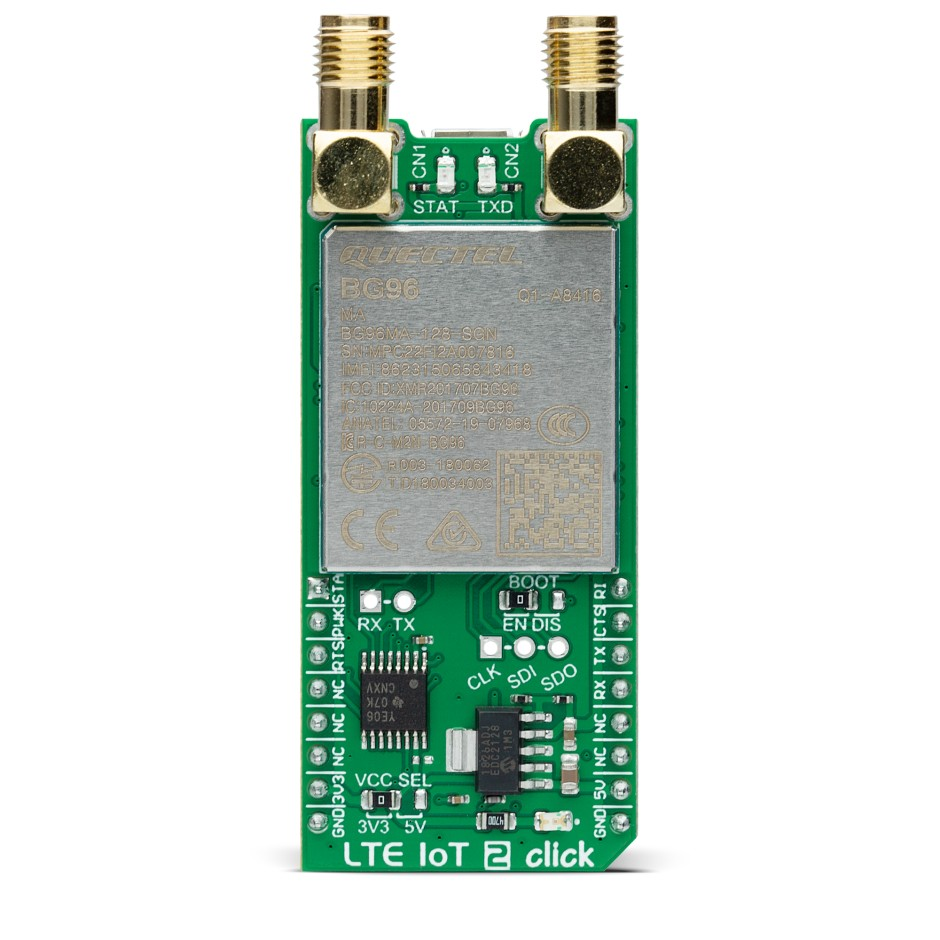
\includegraphics[width=.4\textwidth]{./Figures/moduloBG96.jpg}
	\caption{Modulo LTE IOT 2 CLICK.}
	\label{fig:modulo LTE IOT}
\end{figure}

\subsection{Sensor AHT10}
AHT10 es un sensor que permite obtener lecturas de temperatura y humedad, es de bajo costo y excelente rendimiento. El sensor es muy versátil, puede sustituir a los sensores DHT11, SHT20 y AM2302, debido a su estabilidad en entornos más hostiles. Utiliza este sensor en aplicaciones de control automático de temperatura, aire acondicionado, estaciones meteorológicas, aplicaciones en el hogar, regulador de humedad y temperatura.
\begin{figure}[htbp]
	\centering
	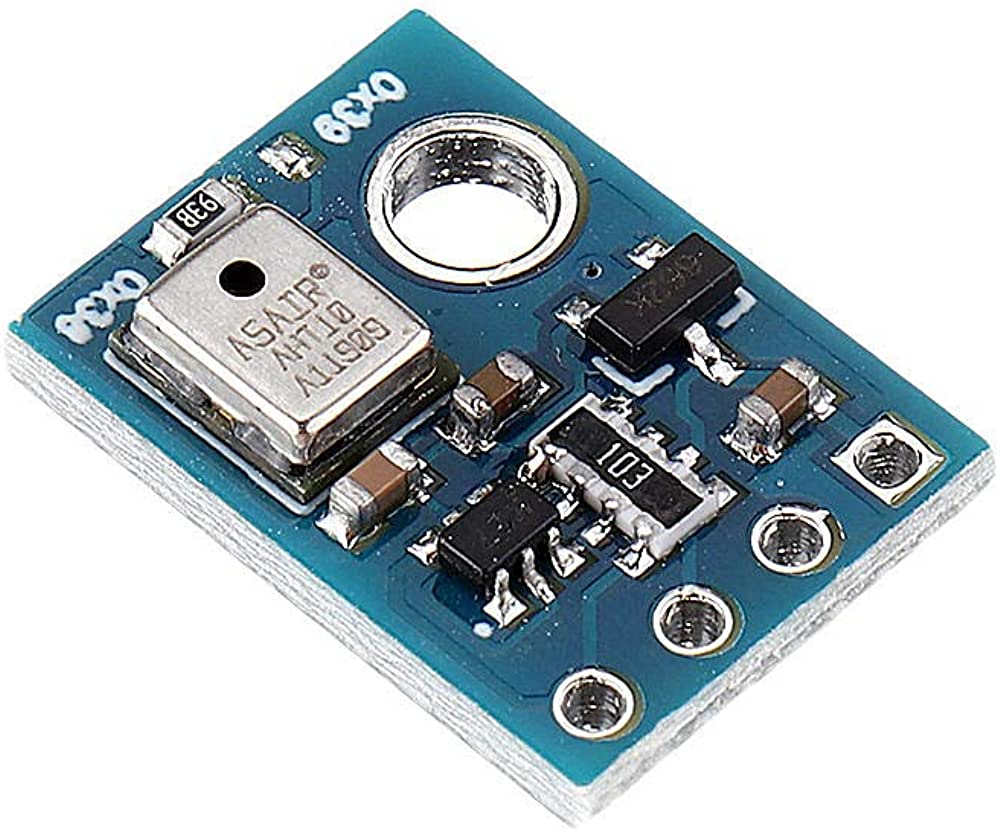
\includegraphics[width=.4\textwidth]{./Figures/aht10.jpg}
	\caption{Modulo LTE IOT 2 CLICK.}
\end{figure}

\subsection{Sensor ML8511}

El módulo ML8511 es un sensor de luz ultravioleta (UV), entrega una señal de voltaje analógica que depende de la cantidad de luz UV que detecta. Sensor ideal para proyectos de monitoreo de condiciones ambientales como el índice UV, Aplicaciones Meteorológicas, cuidado de la piel, medición industrial de nivel UV.
El sensor ML8511 detecta luz con una longitud de onda entre 280-390 nm, este rango cubre tanto al espectro UV-B como al UV-A. La salida analógica está relacionada linealmente con la intensidad UV (mW/cm2). Esta señal analógica puede ser conectada a un microcontrolador para ser convertido por un ADC y así trabajar con la medición. 
\begin{figure}[htbp]
	\centering
	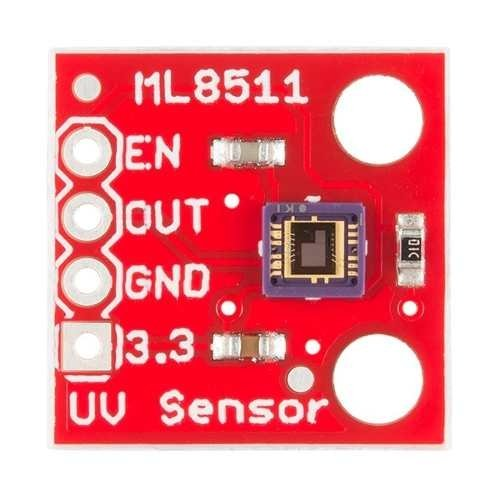
\includegraphics[width=.4\textwidth]{./Figures/ml8511.jpg}
	\caption{Modulo LTE IOT 2 CLICK.}
\end{figure}
\subsection{Sensor de Humedad de Suelo HL-69 (Resistivo)}
El módulo HL-69, un sensor de humedad de suelo resulta ser otro módulo que utiliza la conductividad entre dos terminales para determinar ciertos parámetros relacionados a agua, líquidos y humedad.
\begin{figure}[htbp]
	\centering
	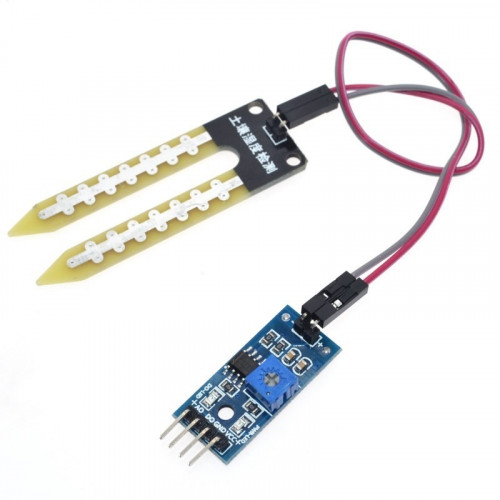
\includegraphics[width=.4\textwidth]{./Figures/sensordehumedad.jpg}
	\caption{Modulo LTE IOT 2 CLICK.}
\end{figure}

\section{Herramientas de software y testing utilizados}
\subsection{STM CUBEIDE}
STM32CubeIDE es una herramienta de desarrollo multi-OS todo en uno, que forma parte del ecosistema de software STM32Cube.STM32CubeIDE es una plataforma de desarrollo C/C++ avanzada con funciones de configuración de periféricos, generación de código, compilación de código y depuración para microcontroladores y microprocesadores STM32. Se basa en el marco Eclipse  y la cadena de herramientas GCC para el desarrollo y GDB para la depuración. Permite la integración de los cientos de plugins existentes que completan las funcionalidades del IDE de Eclipse .

STM32CubeIDE integra las funcionalidades de configuración y creación de proyectos de STM32 de STM32CubeMX para ofrecer una experiencia de herramienta todo en uno y ahorrar tiempo de instalación y desarrollo.

\subsection{FreeRTOS}
\label{subsec:FreeRTOS}
FreeRTOS es un sistema operativo en tiempo real (RTOS) líder en el mercado para microcontroladores y pequeños microprocesadores. Distribuido libremente bajo la licencia de código abierto del MIT, FreeRTOS incluye un núcleo y un conjunto creciente de bibliotecas adecuadas para su uso en todos los sectores de la industria.
FreeRTOS está diseñado con énfasis en la confiabilidad, la accesibilidad y la facilidad de uso.
\begin{figure}[htbp]
	\centering
	
\includegraphics[width=0.6\textwidth]{./Figures/logo_FreeRTOS.jpg}
	\caption{Logo FreeRTOS.}
	\label{fig:FreeRTOS}
\end{figure}
\subsection{CEEDLING}
eedling es un sistema de compilación para proyectos C que es algo así como una extensión del sistema de compilación Rake (make-ish) de Ruby. Ceedling está dirigido principalmente al desarrollo basado en pruebas en C y está diseñado para reunir CMock, Unity y CException, otros tres increíbles proyectos de código abierto sin los que no puede vivir si está creando maravillas en el lenguaje C. Con el fin de difundir la genialidad, Ceedling es un artilugio extensible con un buen mecanismo de complemento.

Ceedling es nuestra última pieza asombrosa diseñada para reunir todas nuestras ventajas para desarrolladores de C en algo más cohesivo.
\section{Protocolos de Comunicación}
\subsection{UART}
UART (universal asynchronous receiver / transmitter, por sus siglas en inglés) define un protocolo o un conjunto de normas para el intercambio de datos en serie entre dos dispositivos. UART es sumamente simple y utiliza solo dos hilos entre el transmisor y el receptor para transmitir y recibir en ambas direcciones. Ambos extremos tienen una conexión a masa. La comunicación en UART puede ser simplex(los datos se envían en una sola dirección), semidúplex(cada extremo se comunica, pero solo uno al mismo tiempo), o dúplex completo(ambos extremos pueden transmitir simultáneamente). En UART, los datos se transmiten en forma de tramas.
\subsection{I2C}
El bus de comunicaciones I2C  es un protocolo que se efectúa por medio de dos hilos. A través de estos dos hilos pueden conectarse diferentes dispositivos donde algunos de ellos serán maestros en cuanto muchos otros dispositivos serán esclavos.
\subsection{MQTT}
MQTT es un protocolo de mensajería estándar de OASIS para Internet de las cosas (IoT). Está diseñado como un transporte de mensajería de publicación/suscripción extremadamente liviano que es ideal para conectar dispositivos remotos con un espacio de código pequeño y un ancho de banda de red mínimo. MQTT hoy en día se utiliza en una amplia variedad de industrias, como la automotriz, la manufactura, las telecomunicaciones, el petróleo y el gas, etc.

\begin{figure}[htbp]
	\centering
	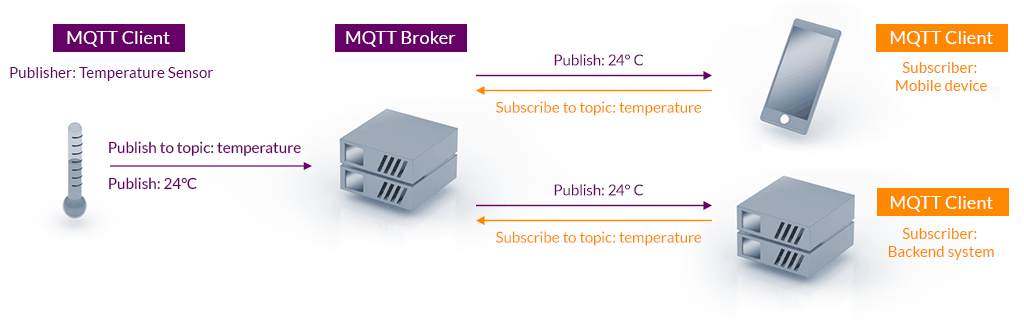
\includegraphics[width=1\textwidth]{./Figures/mqtt-publish-subscribe.png}
	\caption{Arquitectura de publicación/suscripción de MQTT.}
\end{figure}
\section{Plataformas IoT}
\subsection{Ubidots}
Ubidots una plataforma de IoT (Internet de las cosas) que habilita la toma de decisiones a empresas de integración de sistemas a nivel global. Este producto permite enviar datos de sensores a la nube, configurar tableros y alertas, conectarse con otras plataformas, usar herramientas de analítica y arrojar mapas de datos en tiempo real.
Ubidots es una plataforma en la nube para el Internet de las Cosas (IoT) que ofrece todas las herramientas necesarias que permite a las empresas desplegar soluciones IoT, ahorrarse mucho tiempo y dinero a la hora de salir al mercado y poder tomar mejores decisiones basadas en datos.En la figura se muestra un ejemplo una interfaz gráfica en ubidots.
\begin{figure}[htbp]
	\centering
	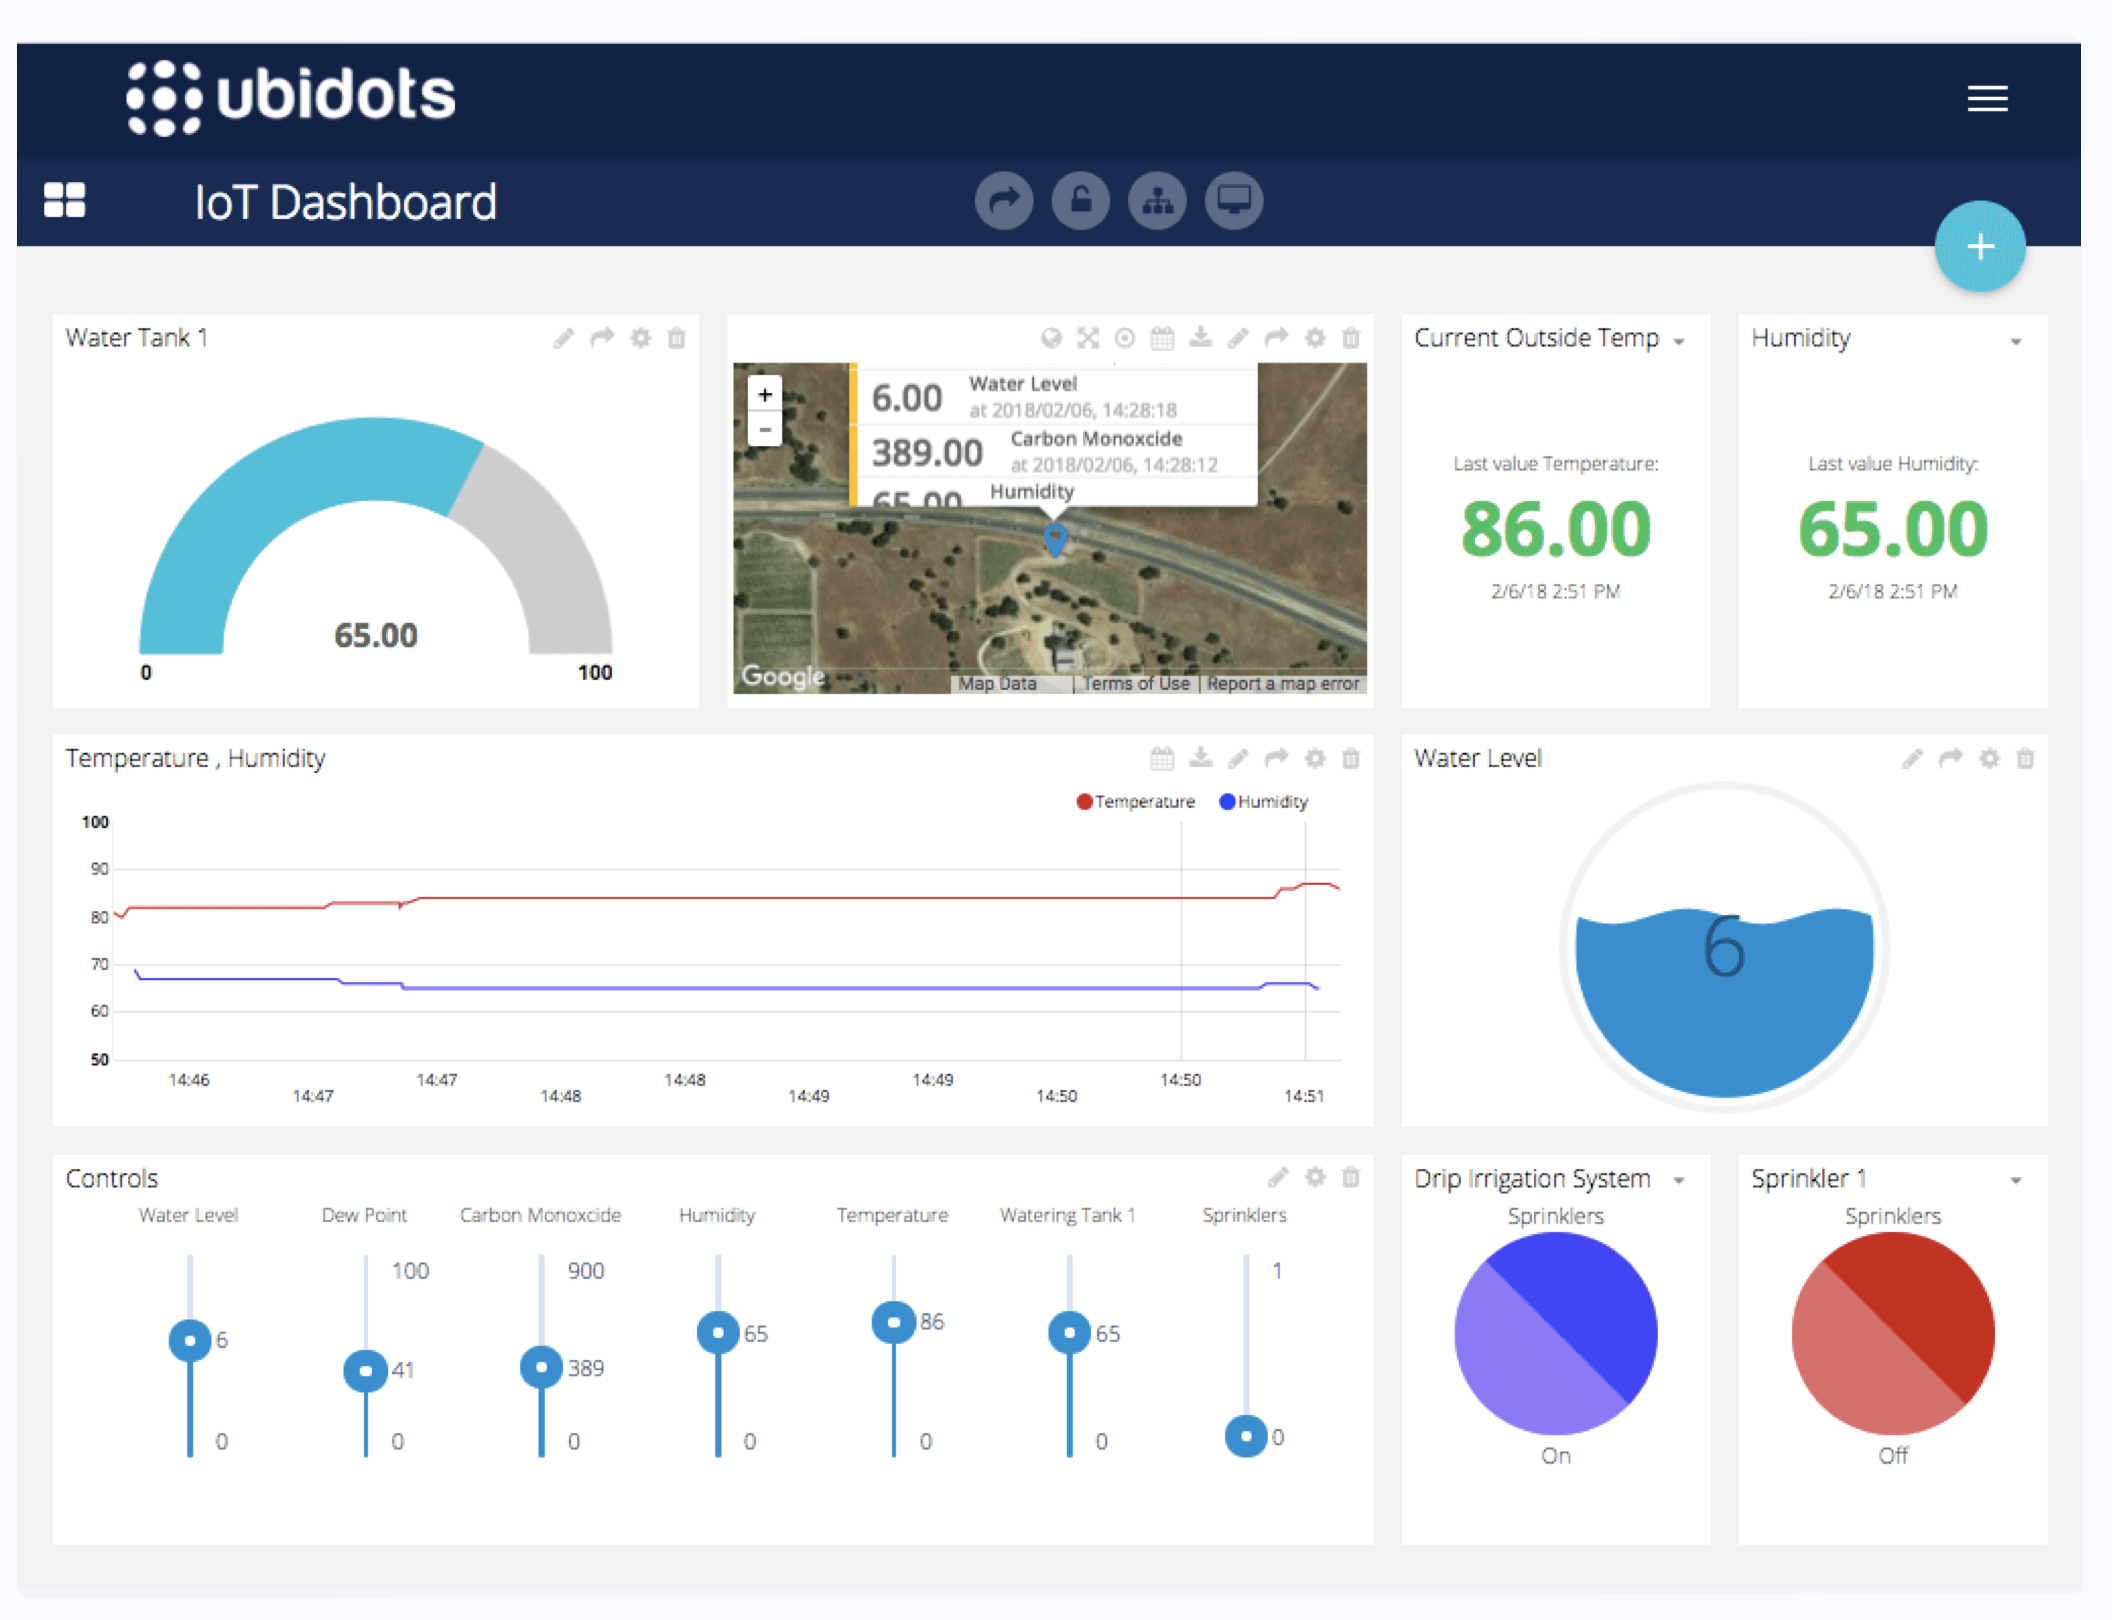
\includegraphics[width=0.6\textwidth]{./Figures/ubidots.png}
	\caption{Ejemplo Interfaz Gráfica Ubidots.}
\end{figure}
\subsection{ThingsBoard}
ThingsBoard es una plataforma IoT de código abierto para la recopilación, el procesamiento, la visualización y la gestión de dispositivos de datos.
Permite la conectividad de dispositivos a través de protocolos IoT estándar de la industria: MQTT, CoAP y HTTP, y admite implementaciones en la nube y locales. ThingsBoard combina escalabilidad, tolerancia a fallas y rendimiento para que nunca pierda sus datos.
\begin{figure}[htbp]
	\centering
	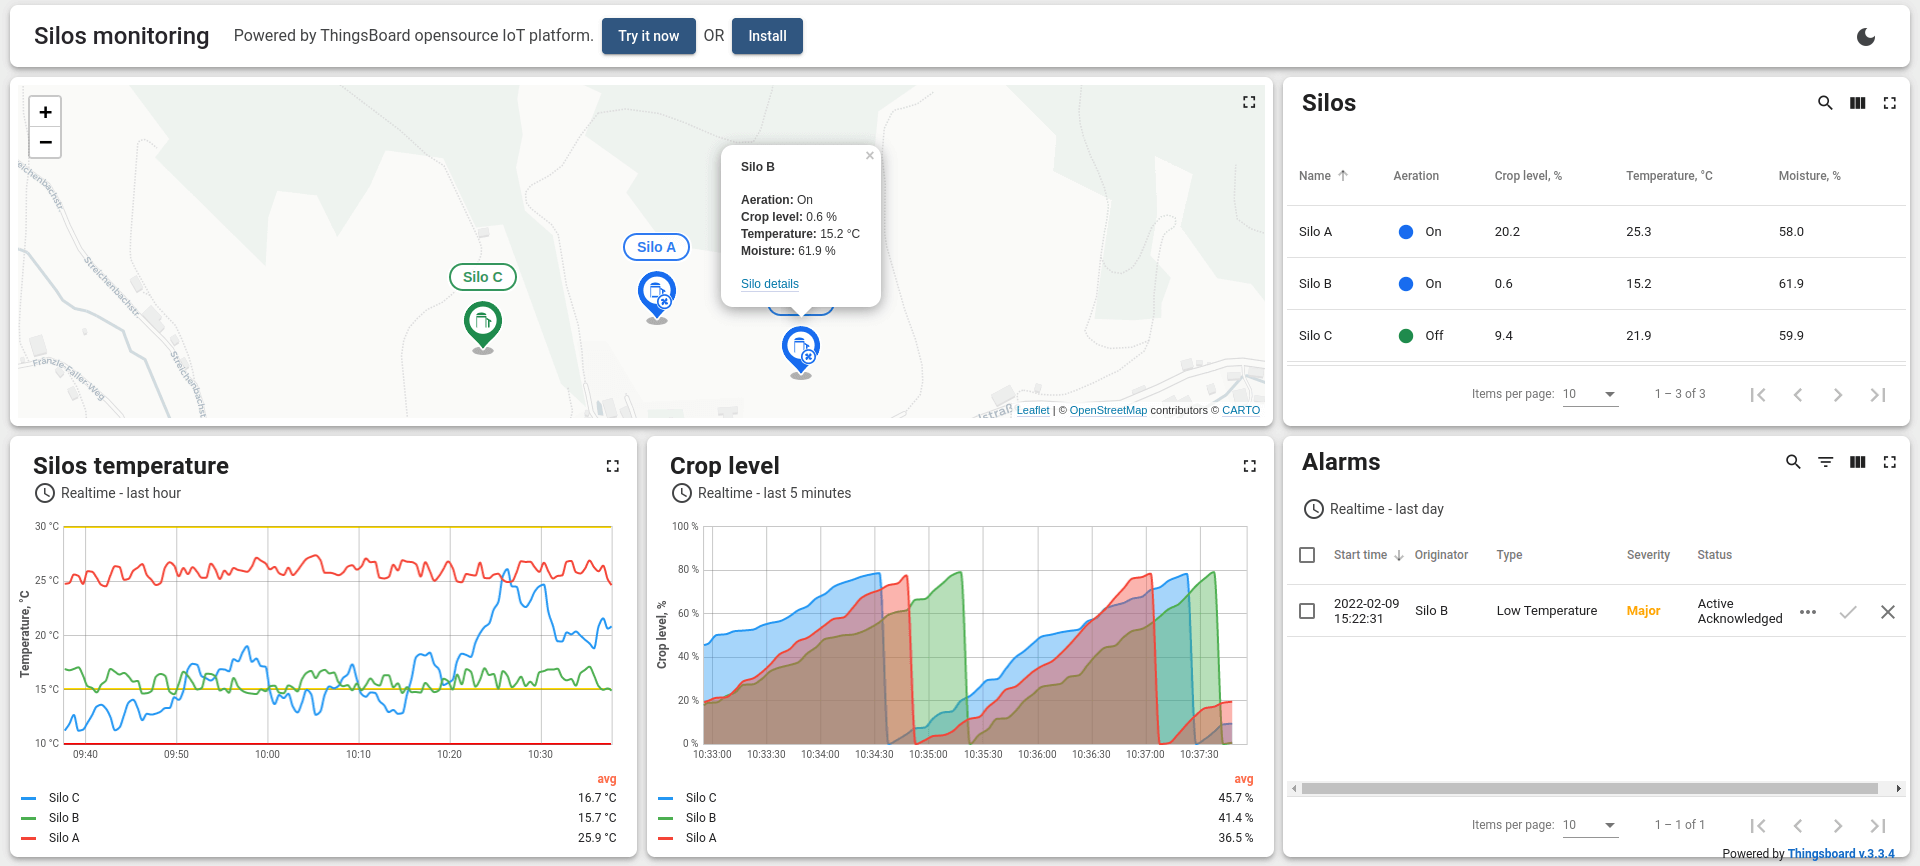
\includegraphics[width=0.8\textwidth]{./Figures/thingsboard.png}
	\caption{Ejemplo Interfaz Gráfica ThingsBoard.}
\end{figure} 

\chapter{Diseño e implementación} % Main chapter title
En este capítulo se abordará la descripción de la arquitectura general del sistema, arquitectura del firmware, código de los controladores desarrollados, desarrollo del hardware y la configuración de la plataforma IoT.
\label{Chapter3} % Change X to a consecutive number; for referencing this chapter elsewhere, use \ref{ChapterX}

\definecolor{mygreen}{rgb}{0,0.6,0}
\definecolor{mygray}{rgb}{0.5,0.5,0.5}
\definecolor{mymauve}{rgb}{0.58,0,0.82}

%%%%%%%%%%%%%%%%%%%%%%%%%%%%%%%%%%%%%%%%%%%%%%%%%%%%%%%%%%%%%%%%%%%%%%%%%%%%%
% parámetros para configurar el formato del código en los entornos lstlisting
%%%%%%%%%%%%%%%%%%%%%%%%%%%%%%%%%%%%%%%%%%%%%%%%%%%%%%%%%%%%%%%%%%%%%%%%%%%%%
\lstset{ %
  backgroundcolor=\color{white},   % choose the background color; you must add \usepackage{color} or \usepackage{xcolor}
  basicstyle=\footnotesize,        % the size of the fonts that are used for the code
  breakatwhitespace=false,         % sets if automatic breaks should only happen at whitespace
  breaklines=true,                 % sets automatic line breaking
  captionpos=b,                    % sets the caption-position to bottom
  commentstyle=\color{mygreen},    % comment style
  deletekeywords={...},            % if you want to delete keywords from the given language
  %escapeinside={\%*}{*)},          % if you want to add LaTeX within your code
  %extendedchars=true,              % lets you use non-ASCII characters; for 8-bits encodings only, does not work with UTF-8
  %frame=single,	                % adds a frame around the code
  keepspaces=true,                 % keeps spaces in text, useful for keeping indentation of code (possibly needs columns=flexible)
  keywordstyle=\color{blue},       % keyword style
  language=[ANSI]C,                % the language of the code
  %otherkeywords={*,...},           % if you want to add more keywords to the set
  numbers=left,                    % where to put the line-numbers; possible values are (none, left, right)
  numbersep=5pt,                   % how far the line-numbers are from the code
  numberstyle=\tiny\color{mygray}, % the style that is used for the line-numbers
  rulecolor=\color{black},         % if not set, the frame-color may be changed on line-breaks within not-black text (e.g. comments (green here))
  showspaces=false,                % show spaces everywhere adding particular underscores; it overrides 'showstringspaces'
  showstringspaces=false,          % underline spaces within strings only
  showtabs=false,                  % show tabs within strings adding particular underscores
  stepnumber=1,                    % the step between two line-numbers. If it's 1, each line will be numbered
  stringstyle=\color{mymauve},     % string literal style
  tabsize=2,	                   % sets default tabsize to 2 spaces
  title=\lstname,                  % show the filename of files included with \lstinputlisting; also try caption instead of title
  morecomment=[s]{/*}{*/}
}


%----------------------------------------------------------------------------------------
%	SECTION 1
%----------------------------------------------------------------------------------------
\section{Diagrama de bloques general del sistema}

En la figura \ref{fig:Diagrama general del sistema IoT} se muestra el diagrama en bloques general del sistema donde se describe la arquitectura IoT aplicada al trabajo que consta de tres capas: percepción, red y aplicación.

\begin{figure}[h]
	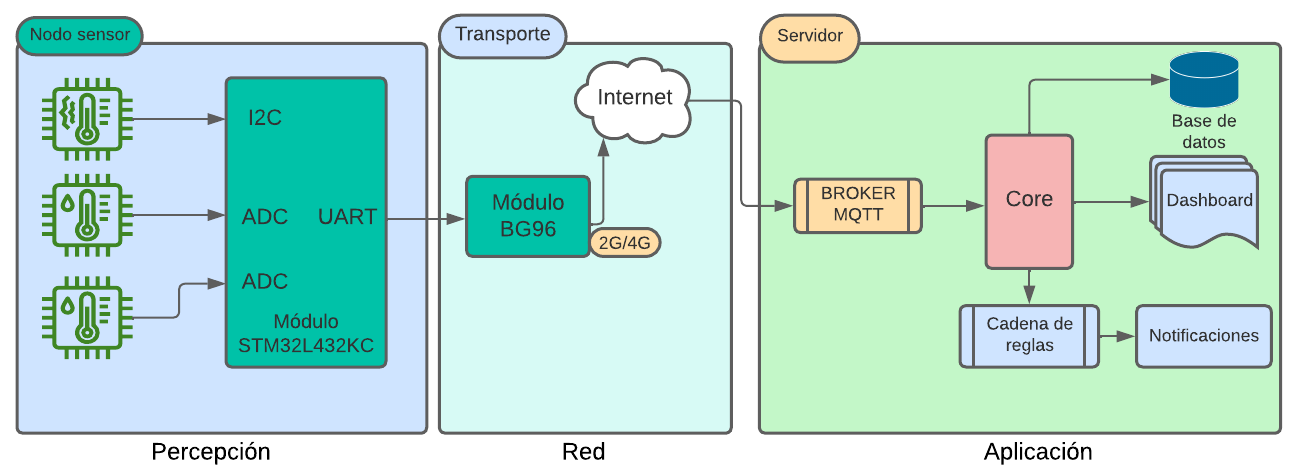
\includegraphics[width=\textwidth, height=8cm]{./Figures/DiagramaDelSistema.png}
	\caption{Diagrama general del sistema IoT.}
	\label{fig:Diagrama general del sistema IoT}
\end{figure}

En cada una de las capas se despliegan tecnologías y componentes de hardware y software. A continuación se describe cada una de las capas.

\begin{itemize}
	\item Capa de percepción: en la capa de percepción se encuentra el nodo sensor que es el encargado de medir las variables físicas, hacer un preprocesamiento y posteriormente enviar los datos a la capa de red. Para su desarrollo se utilizó la tarjeta de prueba STM32L432KC que contiene el firmware del sistema, además, se utilizaron los siguientes sensores: sensor de humedad y temperatura ambiente AHT10, sensor de humedad de suelo HL-69 y el sensor de luz UV ML8511.
  \item Capa de red: en lo que respecta a la conectividad de red, se empleó un módulo Quectel BG96 que es capaz de establecer conexión de manera automática con las redes 2G, 4G y NB-IoT, según las condiciones de red en el lugar de implementación del nodo sensor. Este módulo se comunica con el microcontrolador mediante comandos AT a través del puerto UART.
  \item Capa de aplicación: en la capa de aplicación, se utilizó ThingsBoard como plataforma IoT que brinda los microservicios de broker MQTT como puerta de entrada al servidor, base de datos para el almacenamiento, interfaz gráfica para la visualización de los datos y permite gestionar las alarmas del sistema.
\end{itemize}

\section{Arquitectura de firmware}
El desarrollo del firmware fue la tarea más compleja del trabajo debido a que uno de los objetivos fue lograr un firmware estructurado en capas para facilitar el desarrollo y reducir la complejidad del código. La figura \ref{fig:Capas del firmware} muestra la división en capas del firmware desarrollado.

\begin{figure}[h]
  \centering
	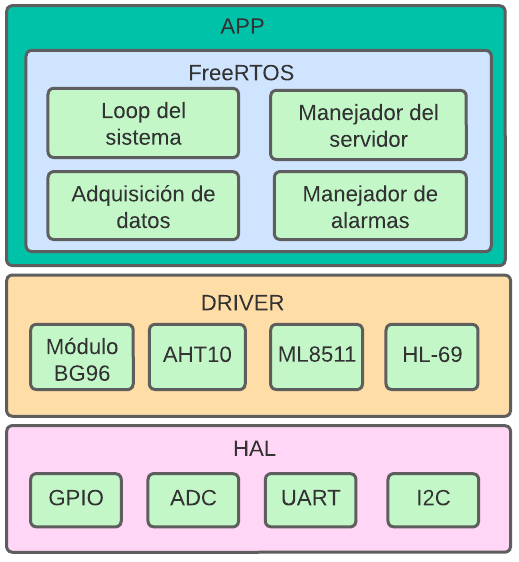
\includegraphics[width=7cm, height=8cm]{./Figures/Capas del firmware.png}
	\caption{Capas del firmware.}
	\label{fig:Capas del firmware}
\end{figure}

\subsection{Capa HAL} 
La capa HAL (\textit{Hardware Abstraction Layer}) proporcionada por el fabricante del microcontrolador  es la más baja del sistema, proporciona a las capas superiores la capacidad de interactuar con los periféricos del  microcontrolador a través de funciones en lenguaje C.
\begin{itemize}
  \item GPIO: la API proporciona funciones  para gestionar las entradas y salidas del microcontrolador. Fueron utilizadas por la capa de APP para el control de los leds de debug y para el encendido y reset del módulo de comunicación.
  \item ADC: proporcionan funciones para la configuración, lectura y escritura de los pines del microcontrolador para trabajar con señales analógicas. Se utilizaron estas funciones para hacer la lectura de los sensores de humedad del suelo y el sensor de luz UV.
  \item UART: brinda funciones para la lectura y escritura del puerto UART del microcontrolador. El firmware utiliza estas funciones para la comunicación con el módulo BG96.
  \item I2C: proporciona funciones para la lectura y escritura por protocolo I2C. El driver del sensor AHT10 utiliza estas funciones para hacer la lectura de los datos.
\end{itemize}

\subsection{Capa drivers} 
La capa drivers (manejador de dispositivos) está compuesta por los manejadores que se desarrollaron para interactuar con el hardware externo al microcontrolador. Se desarrollaron dos drivers que se describen a continuación:
\begin{itemize}
  \item Driver BG96: las funciones más importantes que proporciona el driver son:
  \begin{itemize}
    \item Estado del módulo.
    \item Descripción del módulo.
    \item Configuración APN de la red.
    \item Conexión TCP.
    \item Conexión al broker MQTT.
  \end{itemize}
  \item Driver AHT10: se desarrollo utilizando la hoja de datos del sensor, proporciona funciones de inicialización y lectura de humedad y temperatura obtenidos por el sensor.
\end{itemize}
Para los sensores ML8511 y HL-69 que son sensores analógicos no se desarrollaron drivers, sino que se crearon funciones para convertir el valor analógico entregado a un valor significativo para el usuario con respecto a la variable física medida.
\subsection{Capa aplicación} 
La capa de APP o aplicación  es la de mayor nivel jerárquico. Se desarrolló sobre freeRTOS 
que permite hacer un código más escalable.

Se implementaron cuatro tareas.
\begin{itemize}
    \item Loop del sistema: esta tarea es la que brinda la secuencialidad del sistema.
    \item Manejador del  servidor: se encarga de manejar la conexión a la red y al broker MQTT.
    \item Adquisición de datos: se encarga de hacer la lectura de los sensores.
    \item Manejador de alarmas: esta tarea se encarga de hacer el control de las alarmas del sistema.
\end{itemize}
\clearpage

\section{Desarrollo del firmware}

Para el desarrollo del firmware se utilizó STM32CubeIDE que es el entorno de desarrollo oficial de STMicroelectronic.

El firmware fue desarrollado sobre freeRTOS, se utilizaron algunas de sus funcionalidades como colas, semáforos, tareas e interrupciones.

En la figura \ref{fig:Df inicio firmware}  se muestra en diagrama de flujo de inicialización del firmware.

\begin{figure}[htbp]
  \centering
	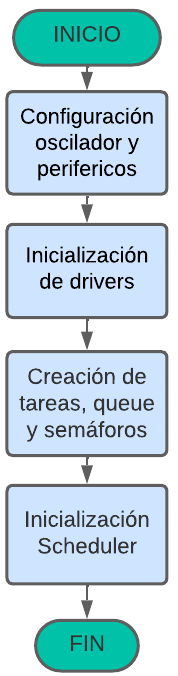
\includegraphics[width=2.5cm, height=9.5cm]{./Figures/DF inicio firmware.png}
	\caption{Diagrama de flujo de inicialización del firmware.}
	\label{fig:Df inicio firmware}
\end{figure}

El firmware comienza realizando la siguiente secuencia de acciones: configuración del hardware del microcontrolador, inicialización de los drivers del hardware externo, creación de los recursos del sistema operativo y finalmente inicialización del scheduler.

Para el control del sistema se crearon cuatro tareas sobre freeRTOS, que se comunican y sincronizan a través de colas y semáforos.

\subsection{Tarea loop del sistema} 

La tarea loop comienza iniciando un timer que se encarga controlar el tiempo de repetición del ciclo de la tarea. Luego la tarea se bloquea. 
Cuando se termina el tiempo del timer, se ejecuta el handler de la interrupción desbloqueando la tarea loop. La tarea envía un evento a cola de adquisición de datos para realizar la lectura  de  los sensores y un evento a cola que maneja la conexión  para levantar el servidor. Posteriormente la tarea comprueba si se logró levantar una conexión. Si la conexión existe la tarea manda un evento  por la cola del servidor para que se envíen los datos al broker MQTT. Luego la tarea  envía un evento a la cola de alarmas para mandar los sms de las alarmas activas del sistema. Finalmente después de monitorear  las alarmas la tarea manda un evento a la cola de servidor para la desconexión. Al finalizar el ciclo de la tarea, inicia el timer nuevamente y manda al microcontrolador a modo de bajo consumo para ahorrar energía.

\begin{figure}[h]  
\centering
	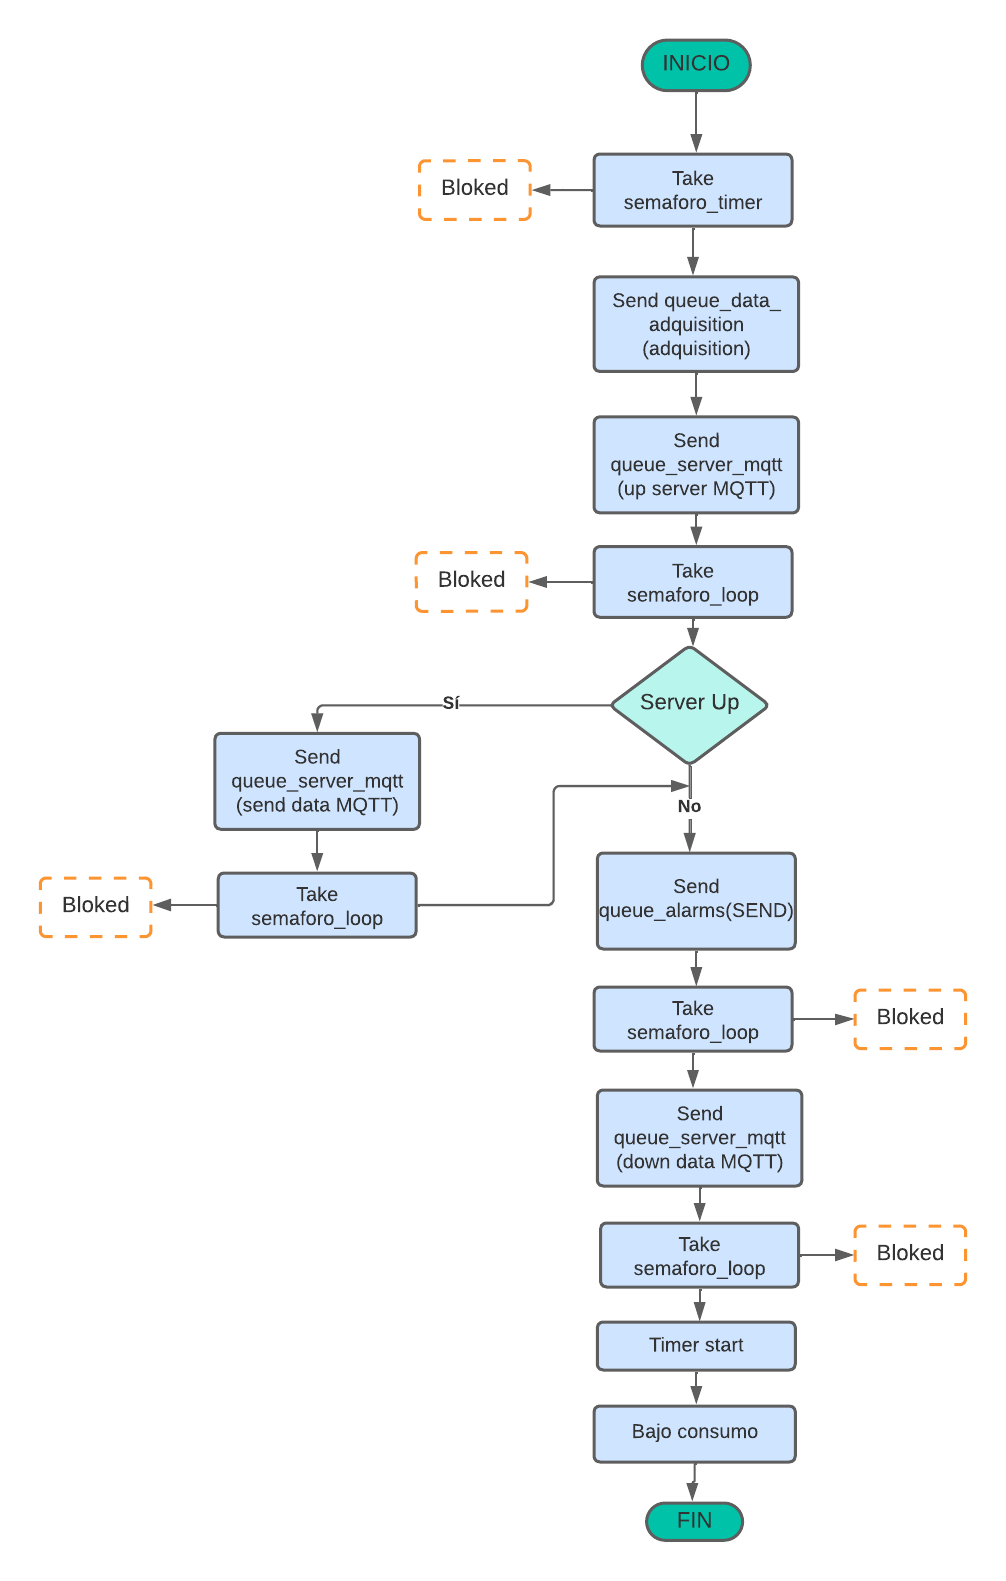
\includegraphics[width=12cm, height=16cm]{./Figures/DF task loop.png}
	\caption{Diagrama de flujo de la tarea loop.}
	\label{fig:Df tarea loop sistema}
\end{figure}

\subsection{Tarea adquisición de datos} 
La figura \ref{fig:Df tarea adquisicion} muestra el diagrama de flujo de la tarea de adquisición de datos. La tarea inicia revisando si hay datos en la cola de adquisición. Si existen datos se realiza la lectura de todos los sensores, para posteriormente enviar los  valores leídos por la cola de datos y alarmas. Si no hay datos en la cola la tarea se bloquea. 

\begin{figure}[h]
  \centering
	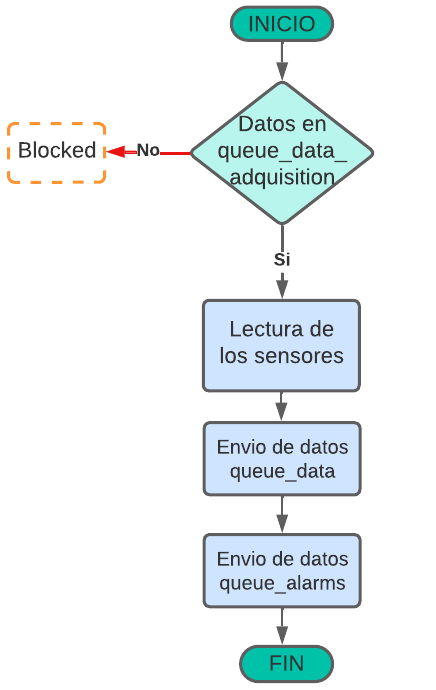
\includegraphics[width=5cm, height=7cm]{./Figures/DF task adquisicion.png}
	\caption{Diagrama de flujo tarea de adquisición de datos.}
	\label{fig:Df tarea adquisicion}
\end{figure}

\subsection{Tarea manejador de alarmas} 
El control de las alarmas se realiza a través una tarea del sistema operativo, la figura \ref{fig:Df tarea alarmas} muestra el diagrama de flujo de la tarea que maneja las alarmas.

Al entrar al bucle infinito lo primero que realiza la tarea es revisar la cola de alarmas. Si existen datos en la cola, se analiza el evento que contiene el dato recibido. Se tiene dos posibles eventos: monitorear y enviar. Si el evento es monitorear se compara el valor del sensor de humedad con un valor mínimo permitido, si es menor se activa una alarma advierte al sistema que ocurrió esto a través de una variable. Si el evento es enviar se revisa si hay alarmas activas, enviando un mensaje de texto si así fuera. Si no hay datos en la cola de alarmas la tarea se bloquea. 

\begin{figure}[h]
  \centering
	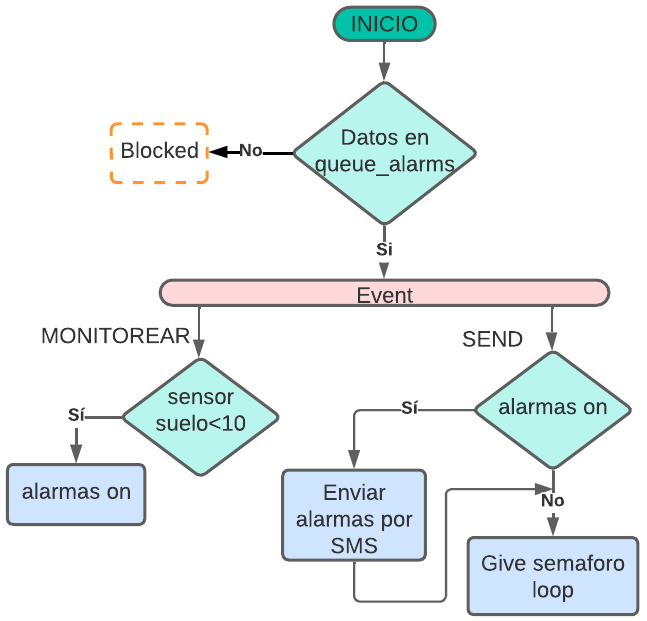
\includegraphics[width=6cm, height=6cm]{./Figures/DF_alarms.png}
	\caption{Diagrama de flujo de la tarea manejador de alarmas.}
	\label{fig:Df tarea alarmas}
\end{figure}

\subsection{Tarea manejador del servidor } 
La tarea comienza esperando datos en la cola del servidor, al llegar datos se analiza el evento que se recibe. Se tiene tres posibles eventos: UP, DOWN y SEND. Si el evento es UP la tarea entra a la máquina de estados que se muestra en la figura \ref{fig:Maquina de estados up servidor} encargada de levantar una conexión con el servidor. Si el evento es DOWN la tarea ejecuta la máquina de estados que se ve en la figura \ref{fig:Maquina de estados dowm servidor} que se encarga de terminar la conexión con el servidor. Si el evento es SEND la tarea obtiene los últimos datos leídos por los sensores, armar la trama y publica los datos al broker MQTT. 
\begin{figure}[h]
  \centering
	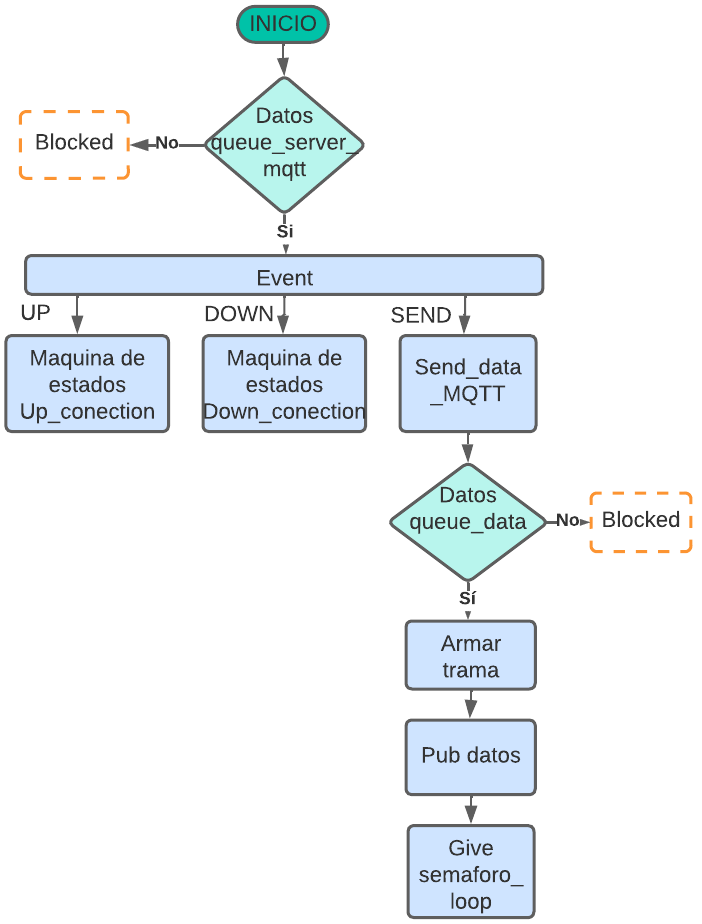
\includegraphics[width=8cm, height=8.5cm]{./Figures/DF general task conection.png}
	\caption{Diagrama de flujo de la tarea conexion server MQTT.}
	\label{fig:Df tarea conexion}
\end{figure}

\begin{figure}[h]
  \centering
  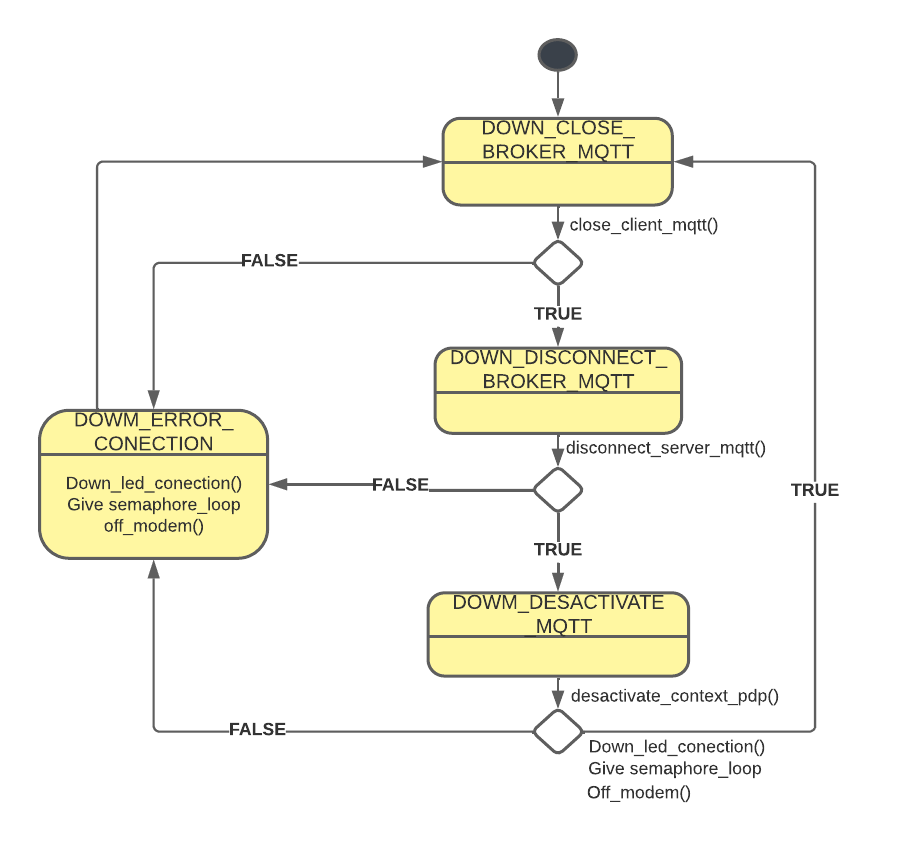
\includegraphics[width=8cm, height=8cm]{./Figures/SM down server.png}
  \caption{Máquina de estados down servidor.}
  \label{fig:Maquina de estados dowm servidor}
\end{figure}
\clearpage
\hspace{0.5cm}

\begin{figure}[t!]
  \centering
	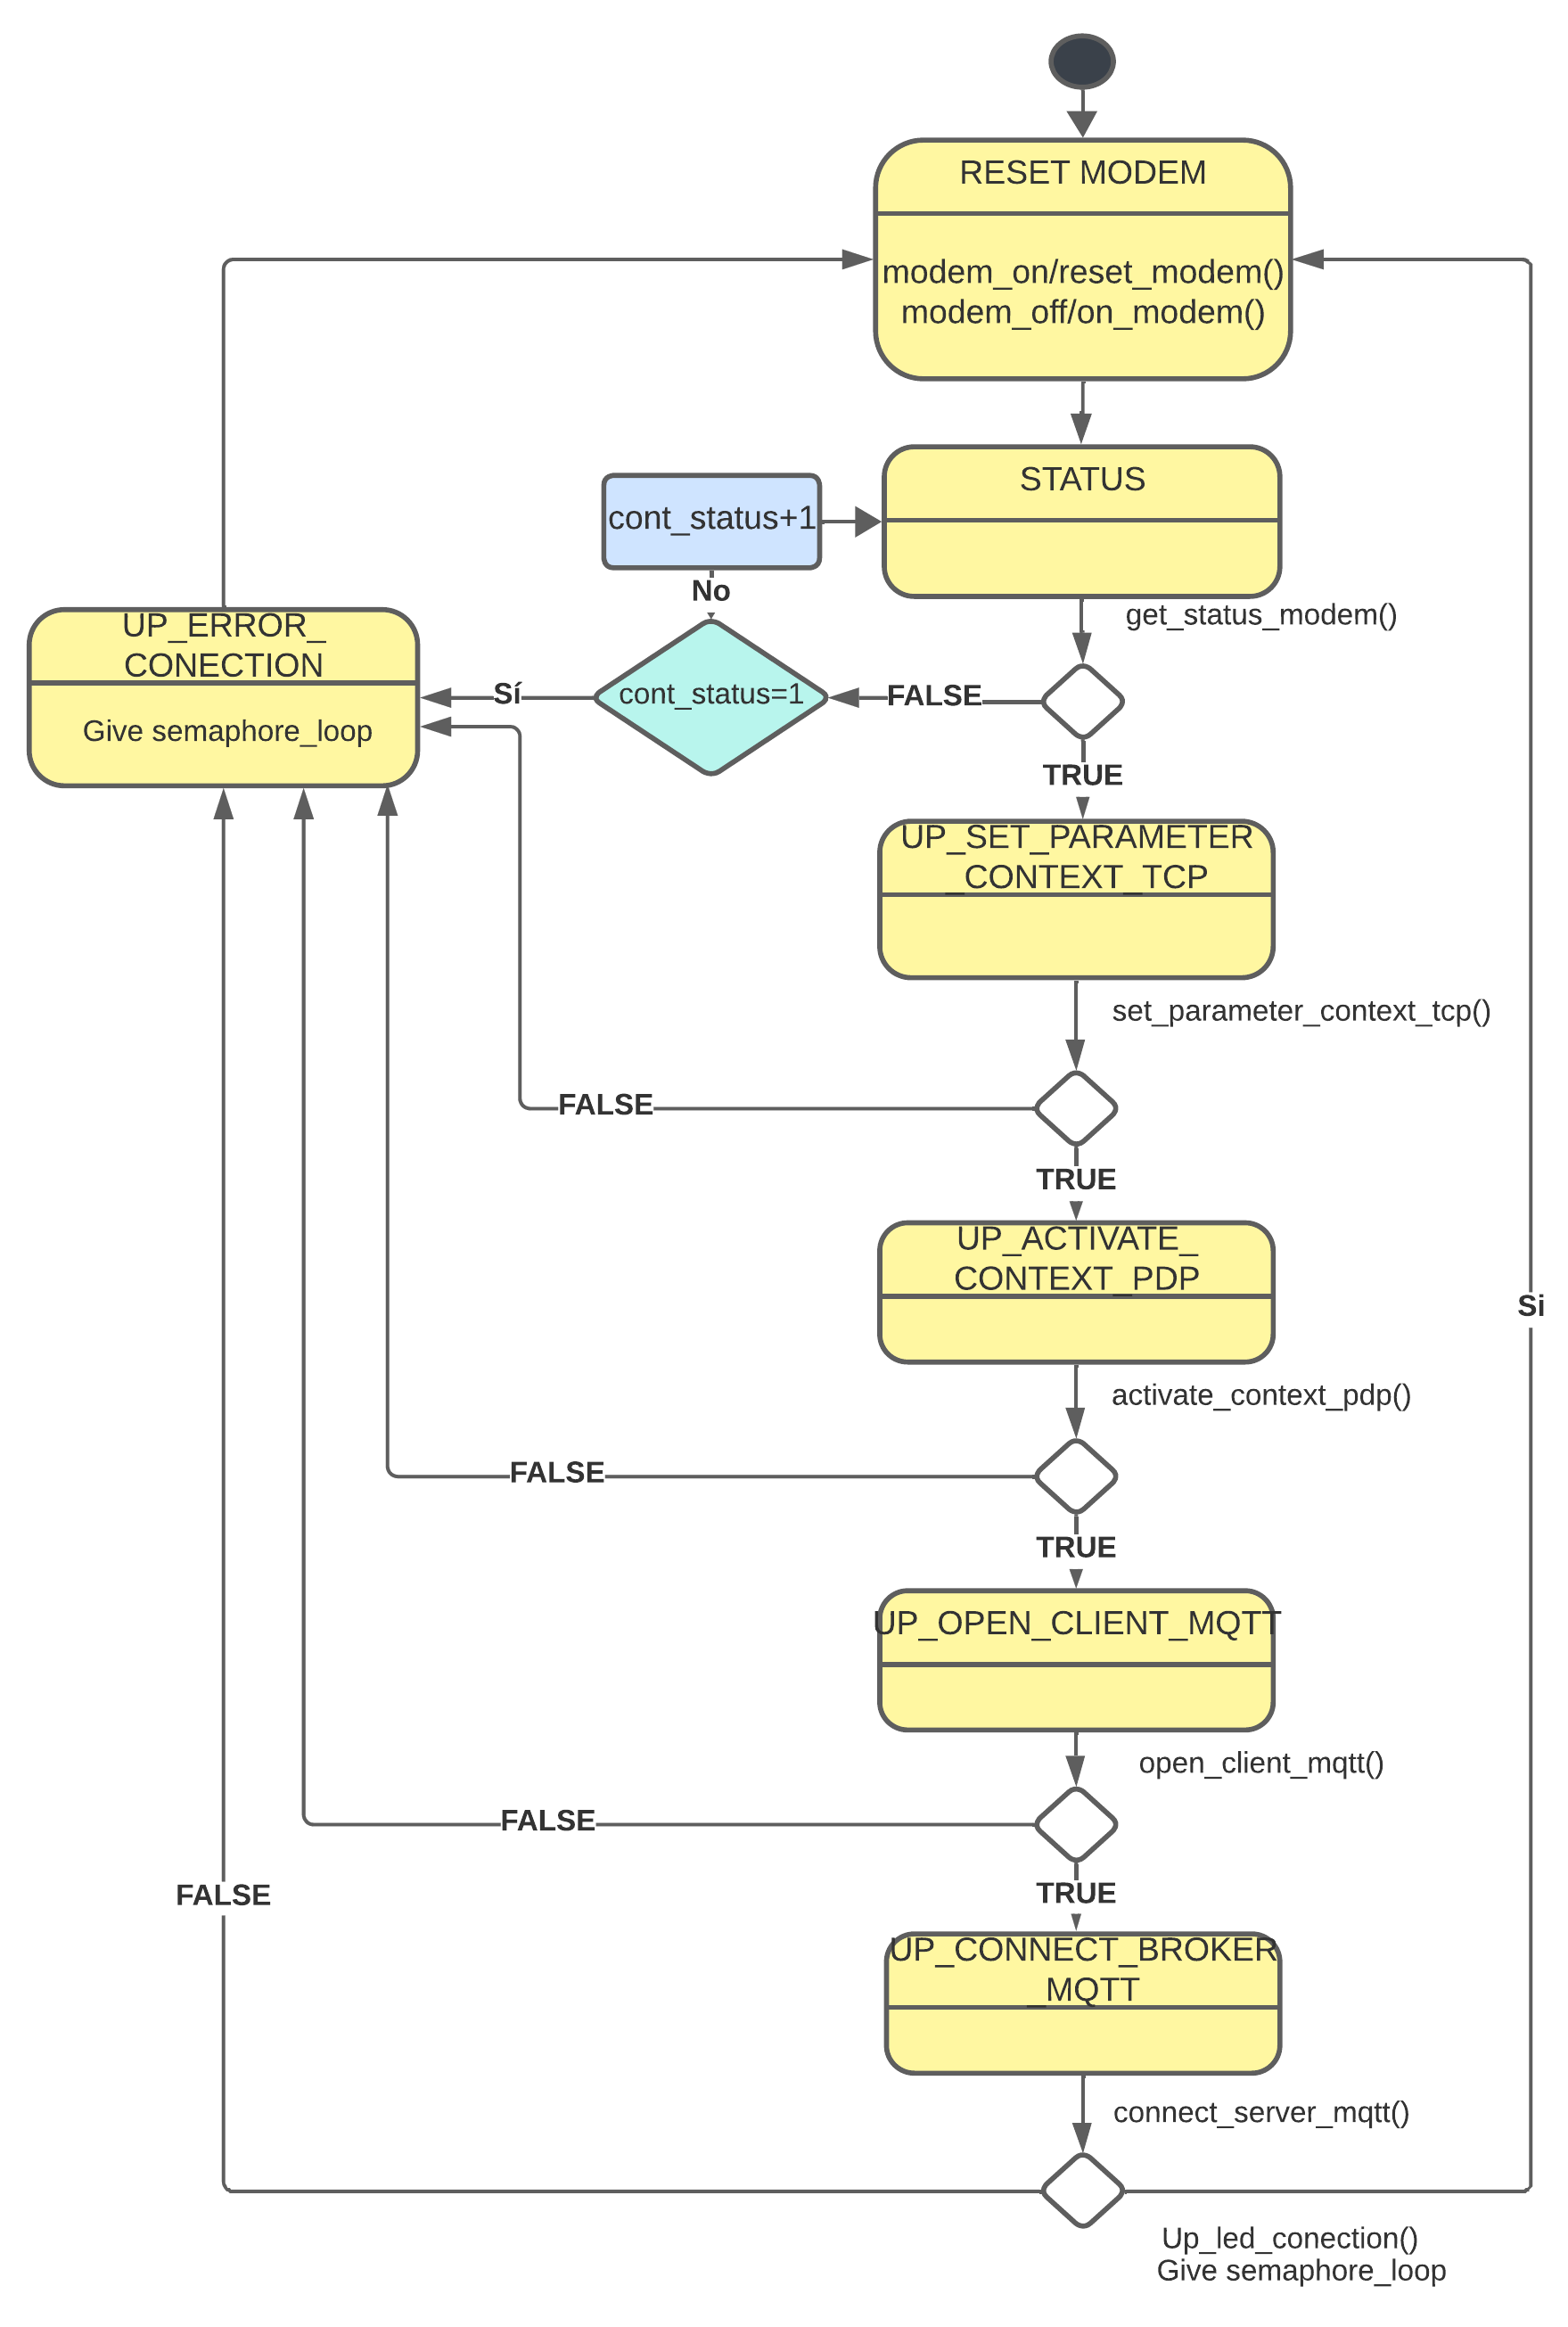
\includegraphics[width=10cm, height=14cm]{./Figures/SM up server.png}
	\caption{Máquina de estados up servidor.}
	\label{fig:Maquina de estados up servidor}
\end{figure}

\section{Controladores implementados}
Se implementaron dos controladores: para el modulo de comunicacion BG96 y para el sensor de humedad y temperatura ambiente AHT10.

\subsection{Controlador sensor AHT10} 

Para la lectura de humedad y temperatura, se desarrolló en el driver las funciones de \emph{aht10\_get\_humedity()} y \emph{aht10\_get\_temperature()} que se muestran en el código \ref{cod:codigo funciones lectura}.
Las funciones comienzan iniciando una medición en el sensor con la función \emph{aht10\_launch\_measurement()}, luego realizan la lectura de los registros del sensor, almacenando los valores de retorno en un buffer. Con los bytes obtenidos se realiza un corrimiento para  obtener los bytes que contienen la información de humedad y temperatura. Finalmente se aplican las fórmulas de las líneas 1 y 2 del código \ref{cod:codigo funciones lectura} para convertir los bytes en valores significativos de las variables físicas.
 
\begin{lstlisting}[label=cod:codigo funciones lectura ,caption=Funciones de lectura de humedad y temperatura.]  % Start your code-block

#define TEMPERATURE(A)                       (int8_t) ((A *0.000191)-50)       
#define HUMEDITY(A)                          (uint8_t) (A *0.000095)        
//Funcion para obtener el valor de la humeda
aht10_status_fnc aht10_get_humedity(aht10_config_t*obj, uint8_t *data)
{
  if (obj== NULL)
  {
    return AHT10_ERROR;
  }
  obj->status_fun=AHT10_ERROR;
  uint8_t bufferRead[6]={0};
  uint32_t data_humedity=0;
  obj->status_fun=aht10_launch_measurement(obj);
  if (obj->status_fun==AHT10_OK)
  {
    obj->status_fun= obj->readI2C(AHT10_ADDRESS_SLAVE,bufferRead,6);
    if (obj->status_fun==AHT10_OK)
    {
      data_humedity=(((uint32_t)bufferRead[1]<<16) | ((uint16_t)bufferRead[2]<<8) | (bufferRead[3]))>>4;
      *data= HUMEDITY(data_humedity);
    }
  }
  return obj->status_fun;
}
//Funcion para obtener el valor de la temperatura 
aht10_status_fnc aht10_get_temperature(aht10_config_t*obj, int8_t *data)
{
  if (obj== NULL)
  {
    return AHT10_ERROR;
  } 
  uint8_t buffer_read[6]={0};
  uint32_t data_temperature=0;
  obj->status_fun=AHT10_ERROR;
  obj->status_fun=aht10_launch_measurement(obj);
  if (obj->status_fun==AHT10_OK)
  {
    obj->status_fun=obj->readI2C(AHT10_ADDRESS_SLAVE ,buffer_read,6);
    if (obj->status_fun==AHT10_OK)
    {
      data_temperature=((uint32_t)(buffer_read[3] & 0x0F)<<16) | ((uint16_t) buffer_read[4]<<8)| buffer_read[5];
      *data= TEMPERATURE(data_temperature);
    }
  }
  return obj->status_fun;
}
\end{lstlisting}

\subsection{ Controlador módulo de comunicación BG96 } 
Se desarrollaron varias funciones para el driver BG96, que permiten configurar el módulo, configurar la red y las más importantes para el trabajo las de conexión, publicación y desconexión al servidor MQTT.

El código \ref{cod:driver bg96} muestra dos funciones desarrolladas en el driver BG96. La función \emph{connect\_server\_mqtt()} utilizada para conectarse al servidor MQTT, internamente lo que hace es mandar el comando que se ve en la línea 6 y esperar la respuesta del módulo, que puede ser un OK o ERROR. La función \emph{publish\_message()} es una de las más utilizadas por el firmware, es la encargada de publicar la trama JSON que contiene los datos de los sensores al tópico configurado inicialmente. 
\begin{lstlisting}[label=cod:driver bg96,caption=Función de conexión y publicación al broker MQTT.]  % Start your code-block

//Funcion para conectarse al servidor MQTT
em_bg96_error_handling connect_server_mqtt(st_bg96_config *self)
  {
    self->ft_resp=FT_BG96_ERROR;
    char cmd[150]={0};
    sprintf(cmd,"AT+QMTCONN=%u,\"%s\",\"%s\",\"%s\"\r",self->self_mqtt.identifier_socket_mqtt,self->self_mqtt.mqtt_client_id,self->self_mqtt.mqtt_username,self->self_mqtt.mqtt_password);
    self->ft_resp=self->send_data_device(cmd,RS_BG96_CERO,self->buffer_resp,10000);
    if (self->ft_resp!=FT_BG96_OK)
    {
      self->last_error=BG96_ERROR_CONNECT_SERVER_MQTT;
    }
    return self->ft_resp;
  }
  //Funcion para publicar un mensaje al topico configurado 
  em_bg96_error_handling publish_message(st_bg96_config *self,char *topic,char *data)
  {
    self->ft_resp=FT_BG96_ERROR;
    char cmd[50]={0};
    char buffer_data[220]={0};
    sprintf(buffer_data,"%s\x1a\r",data);
    sprintf(cmd,"AT+QMTPUB=%u,0,0,0,\"%s\"\r",self->self_mqtt.identifier_socket_mqtt,topic);
    self->ft_resp=self->send_data_device(cmd,RS_BG96_SIGNAL,self->buffer_resp,3000);
    if (FT_BG96_OK==self->ft_resp)
    {
      self->ft_resp=self->send_data_device(buffer_data,RS_BG96_CERO,self->buffer_resp,15000);
      if (self->ft_resp!=FT_BG96_OK)
      {
        self->last_error=BG96_ERROR_PUBLISH_MESSAGE;
      }   
   }
      else self->last_error=BG96_ERROR_PUBLISH_MESSAGE;
      return self->ft_resp;
  }
\end{lstlisting}


Para el envío de mensajes de texto se desarrolló en el driver la función \emph{send\_sms\_bg96()} que recibe como parámetros el número al que se desea mandar el mensaje y el texto del mensaje a enviar. El firmware utiliza esta función para mandar mensajes de alarma al usuario.
El código \ref{cod:funcion de sms} muestra la implementación de la funcion \emph{send\_sms\_bg96()}
\begin{lstlisting}[label=cod:funcion de sms,caption=Función para enviar sms.]  % Start your code-block

//Funcion para enviar mensaje de texto 
em_bg96_error_handling send_sms_bg96(st_bg96_config *self,char*number,char*message)
{
  self->ft_resp=FT_BG96_OK;
  char buffer_message[256];
  char buffer_number[20];
  sprintf(buffer_number,"AT+CMGS=\"%s\"\r",number);
  sprintf(buffer_message,"%s\x1a\r",message);
  
  self->ft_resp=self->send_data_device(buffer_number,RS_BG96_SIGNAL,self->buffer_resp,12000);
  if (FT_BG96_OK==self->ft_resp)
  {
    self->ft_resp=self->send_data_device(buffer_message,RS_BG96_OK,self->buffer_resp,12000);
    if (FT_BG96_OK!=self->ft_resp)
    {
      self->last_error=BG96_ERROR_SEND_SMS;
    }
  }
  return self->ft_resp;
}
\end{lstlisting}

\section{Desarrollo del hardware}

Para el diseño del hardware se empleó KiCad 6.0, una herramienta de diseño que se utilizó durante el desarrollo de la especialización.

\subsection{Esquemático} 
Al ser un prototipo lo que se hizo fue desarrollar un tarjeta donde se puedan ensamblar y conectar los módulos utilizados en el trabajo: módulo de comunicación celular, tarjeta de desarrollo con el microcontrolador y  los módulos sensores.

En la figura \ref{fig:esquematico root} se muestra la página raíz del esquemático del trabajo, está dividida en tres zonas:
\begin{itemize}
  \item Zona 1: índice de las hojas esquemáticas del trabajo.
  \item Zona 2: modelo 3D de la tarjeta desarrollada.
  \item Zona 3: conexiones entre los diferentes hojas esquemáticas .
\end{itemize}

\begin{figure}[h]
  \centering
	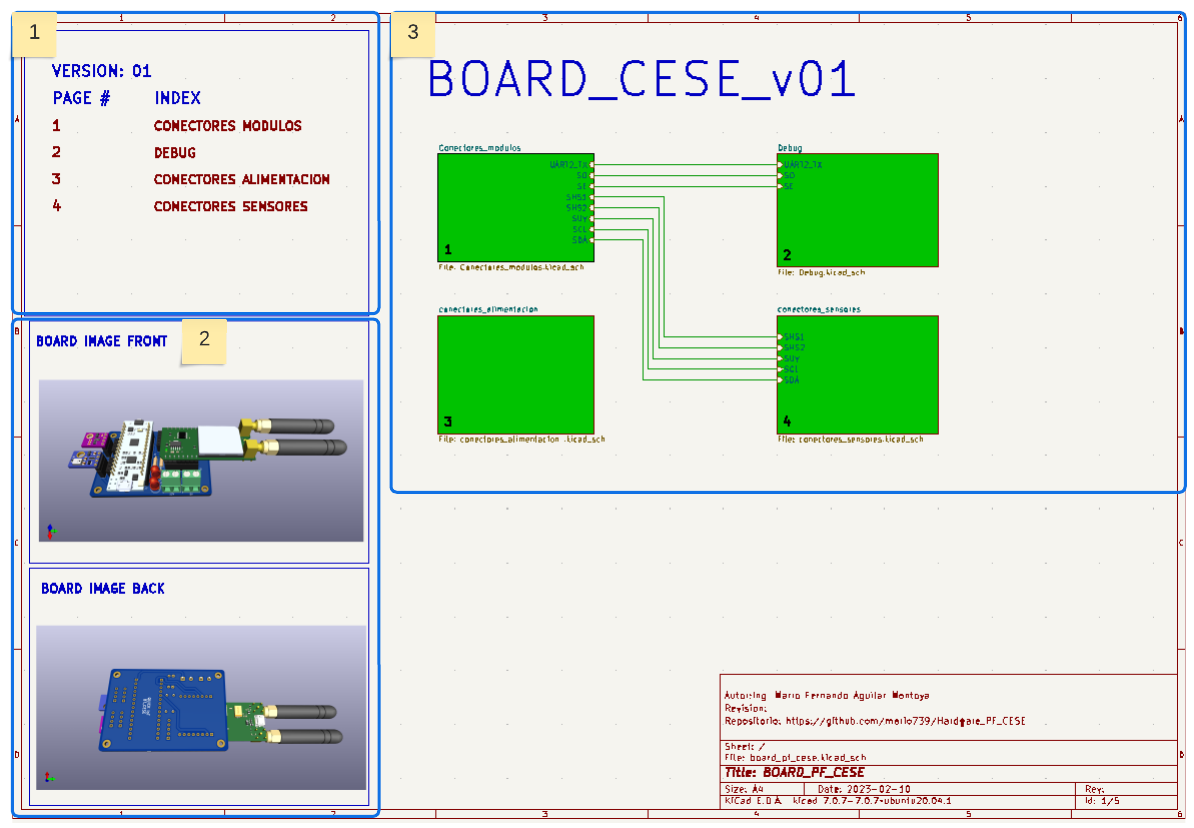
\includegraphics[width=\textwidth, height=8cm]{./Figures/esquematico_raiz.png}
	\caption{Esquemático página raíz.}
	\label{fig:esquematico root}
\end{figure}

En figura \ref{fig:esquematico modulos} se muestran los conectores de los módulos más importantes: el módulo de comunicación BG96, módulo NUCLEO-L432KC y la conexión entre ellos.

\begin{figure}[h]
  \centering
	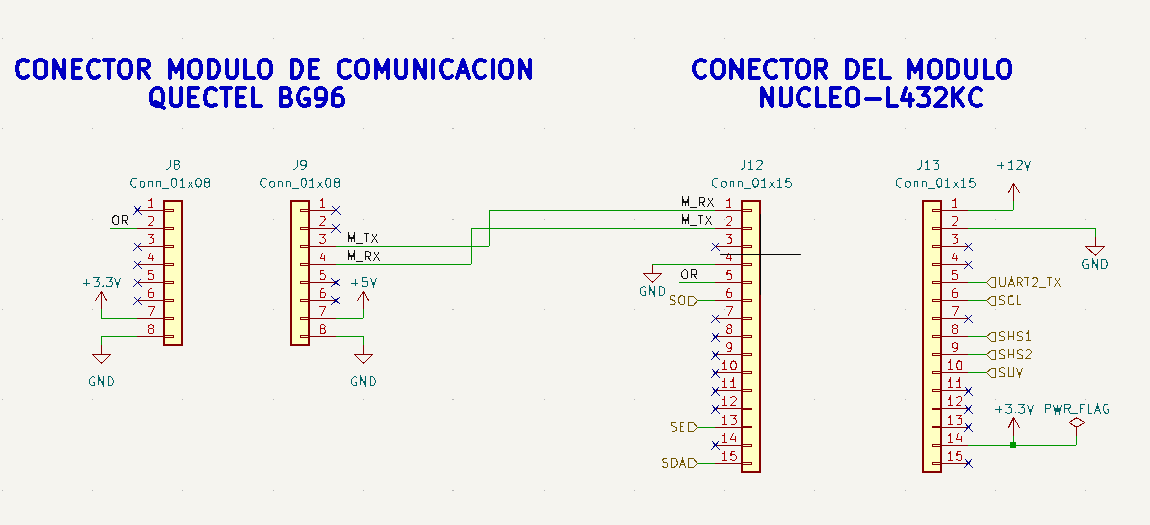
\includegraphics[width=10cm, height=3.5cm]{./Figures/esquematico_modulos.png}
	\caption{Conector módulo BG96 y NUCLEO-L432KC.}
	\label{fig:esquematico modulos}
\end{figure}

Se colocaron dos leds para debug, uno para señalizar si se logró conectar al servidor MQTT y el otro led para señalizar si el sistema entra en un estado de error. Se colocó un conector para una puerto serial por donde el módulo manda la secuencias de comandos que manda y recibe del módulo de comunicación. En la figura \ref{fig:esquematico conectores de debug} se puede ver el circuito.
\begin{figure}[h!]
  \centering
	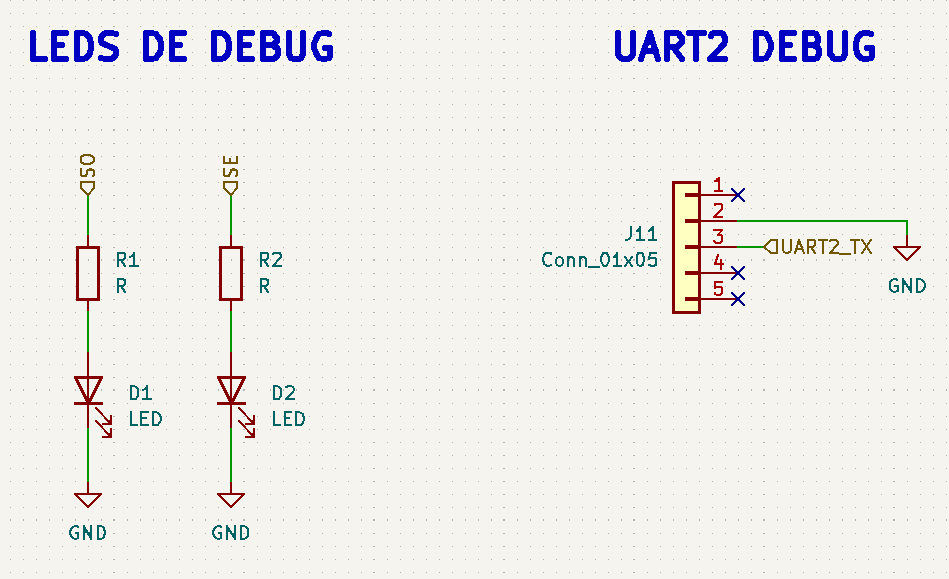
\includegraphics[width=10cm, height=4cm]{./Figures/esquematico_debug.png}
	\caption{Esquemático interfaz de debug.}
	\label{fig:esquematico conectores de debug}
\end{figure}

En la figura \ref{fig:esquematico conectores sensores} se pueden ver los conectores que se colocaron a la placa para conectar los sensores del nodo: sensor de humedad 1, sensor de humedad 2, sensor de luz UV y el sensor de humedad y temperatura ambiente AHT-10.
\begin{figure}[h]
  \centering
	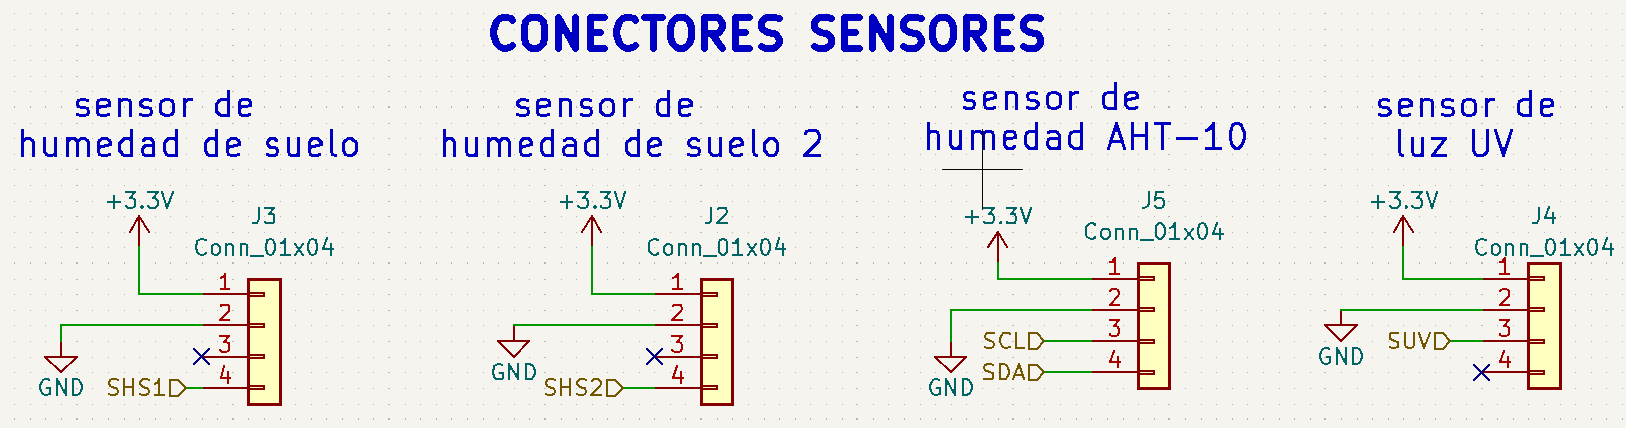
\includegraphics[width=10cm, height=4.5cm]{./Figures/conectores_sensores.png}
	\caption{Esquemático conectores sensores.}
	\label{fig:esquematico conectores sensores}
\end{figure}

Se colocaron dos colectores de alimentación como se muestra en la figura \ref{fig:esquematico conectores alimentacion}, el conector de 12V para alimentar al módulo del microcontrolador y el otro conector para alimentar al módulo de comunicación.
\begin{figure}[h]
  \centering
	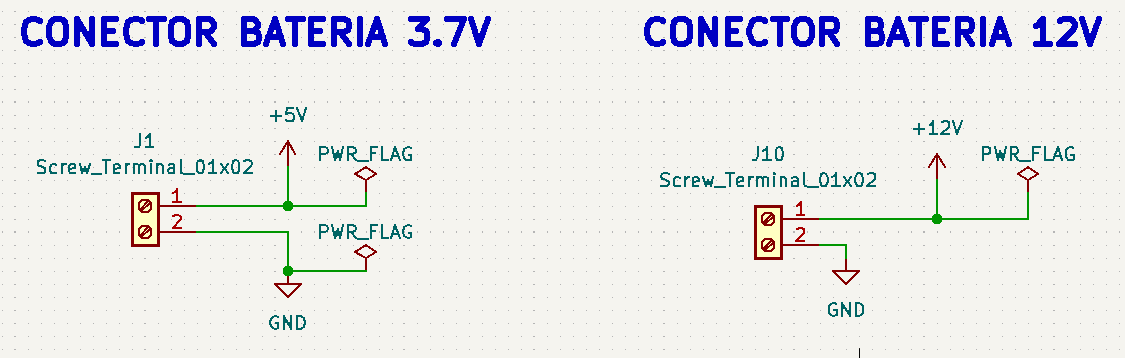
\includegraphics[width=9cm, height=4cm]{./Figures/esquematico_alimentacion.png}
	\caption{Esquemático conectores alimentación.}
	\label{fig:esquematico conectores alimentacion}
\end{figure}

\subsection{PCB del hardware} 
La figura \ref{fig:PCB del proyecto} muestra el circuito impreso diseñado para el proyecto.

\begin{figure}[h!]
  \centering
  \begin{subfigure}[b]{0.28\linewidth}
  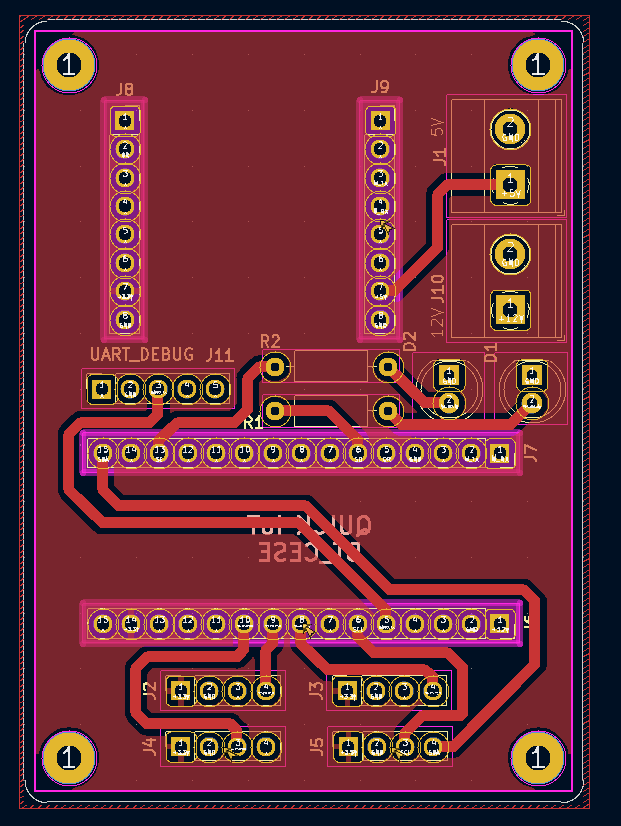
\includegraphics[width=\linewidth]{./Figures/pcb_top.png}
  \caption{Capa top PCB}
  \label{fig:Capa top PCB}
  \end{subfigure}
  \begin{subfigure}[b]{0.27\linewidth}
  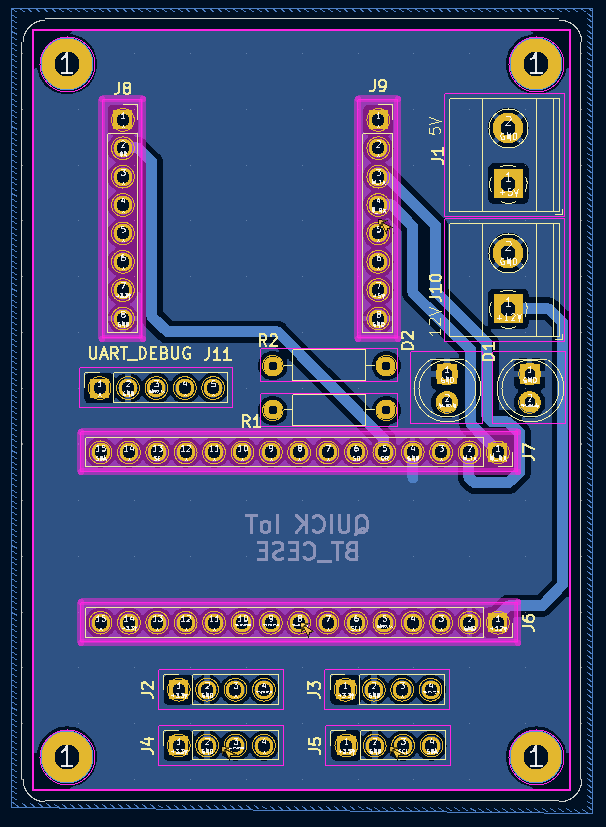
\includegraphics[width=\linewidth]{./Figures/pcb_bot.png}
  \caption{Capa bot PCB}
  \label{fig:Capa bot PCB}
  \end{subfigure}
  \caption{PCB del proyecto.}
  \label{fig:PCB del proyecto}
\end{figure}

En la figura \ref{fig:3D del modulo} se muestra el diseño de la tarjeta del circuito impreso en 3D.
\begin{figure}[h!]
  \centering
	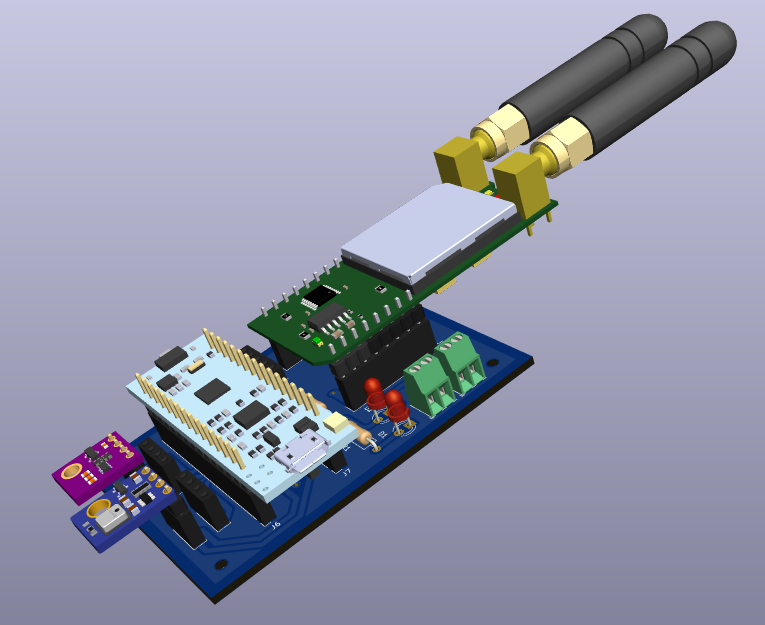
\includegraphics[width=7cm, height=4cm]{./Figures/tarjeta3d.png}
  \caption{Modelo 3D de la tarjeta.}
	\label{fig:3D del modulo}
\end{figure}
\subsection{Fabricación circuito impreso} 
Una vez completado y validado el diseño, se generaron los archivos de fabricación y se mandaron a la empresa JLCPCB parar su producción. La figura \ref{fig:PCB ensamblado} muestra la tarjeta ya ensamblada con los módulos. 
\begin{figure}[h!]
  \centering
	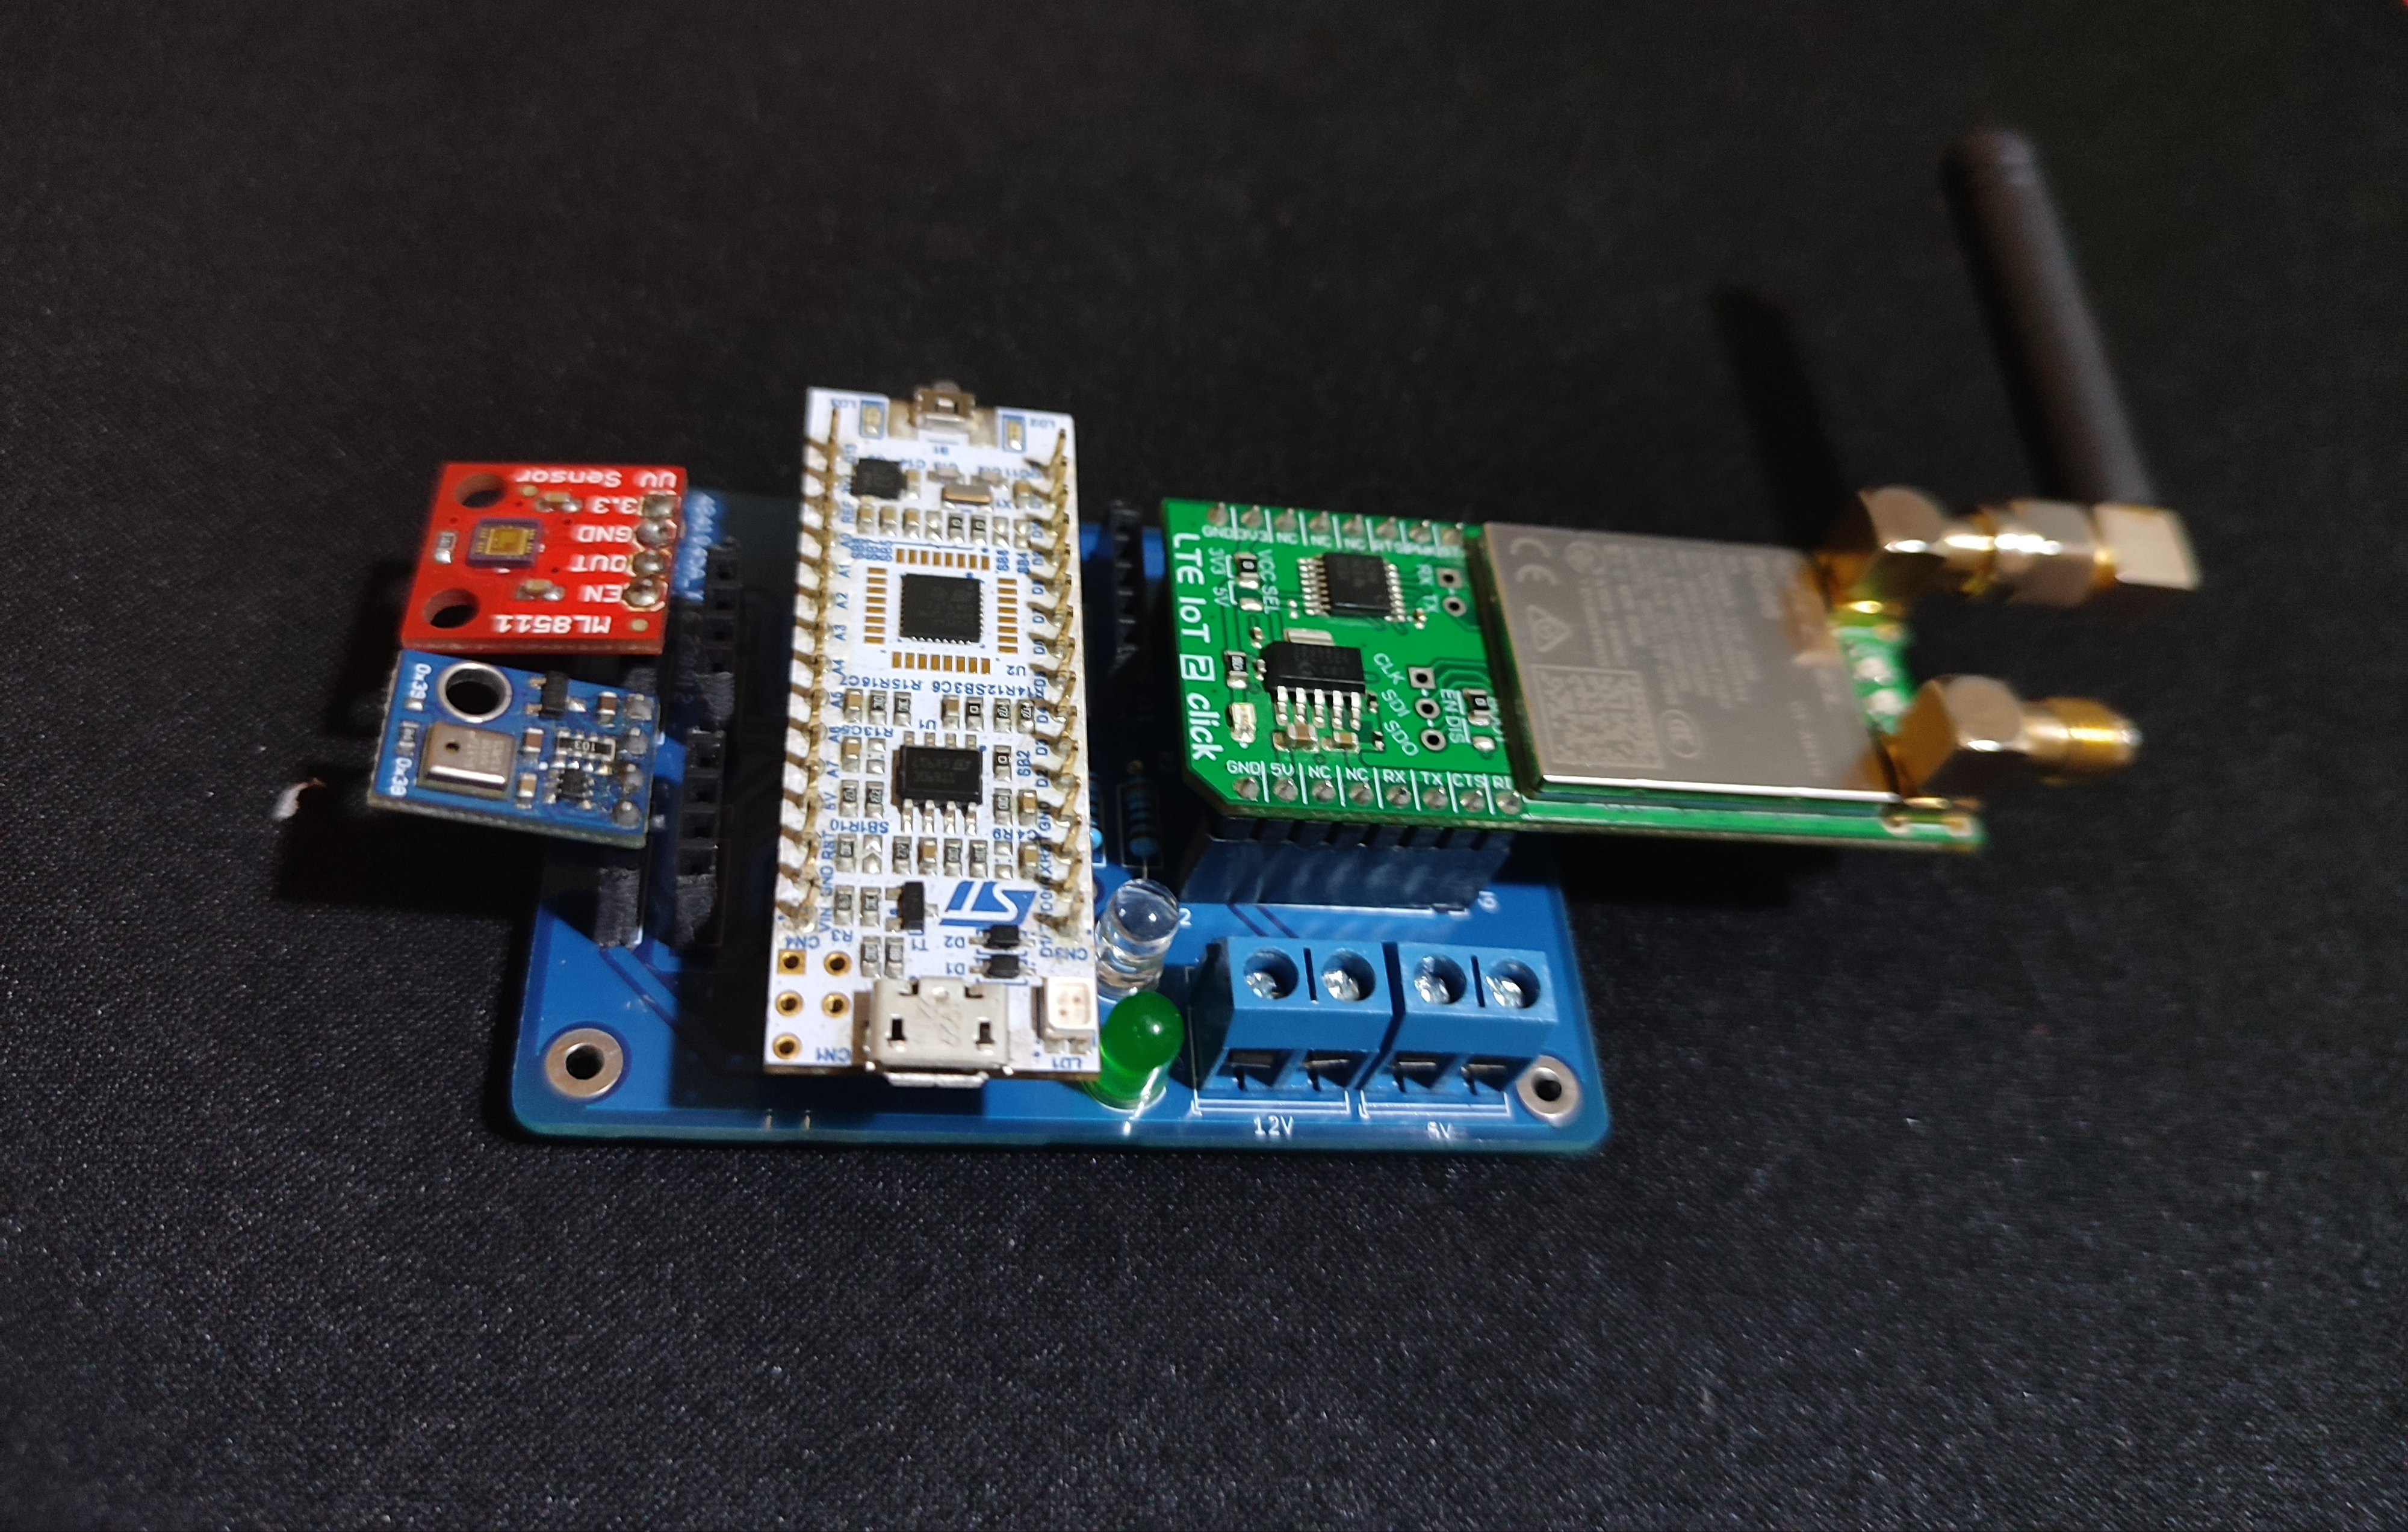
\includegraphics[width=6.5cm, height=4cm]{./Figures/hardware_vistalateral.jpg}
  \caption{PCB ensamblado.}
	\label{fig:PCB ensamblado}
\end{figure}

\section{Paneles de visualización}
La herramienta de visualización de ThingsBoard es muy versátil para el armado de paneles de visualización escalables y altamente configurables.

Se armó un panel de visualización principal que muestra los nodos sensores monitoreados por el sistema y un panel secundario que muestra las variables monitoreadas por cada nodo sensor a través gráficas, tablas, etc.

\subsection{Panel principal} 

En la figura \ref{fig:Panel principal} se aprecia el panel principal de la interfaz gráfica. A continuación se describirán cada zona del panel principal.
El panel está dividido en las siguientes zonas:
\begin{itemize}
  \item Zona 1: listado de todos los nodos sensores implementados y activos, haciendo click en el sensor se navega al panel de visualización secundario.
  \item Zona 2: gráficas que muestra los cambios que van teniendo los valores de las variables medidas por los sensores con respecto al tiempo.
  \item Zona 3: mapa con la ubicación de los nodos sensores implementados.
\end{itemize}

\begin{figure}[h]
  \centering
	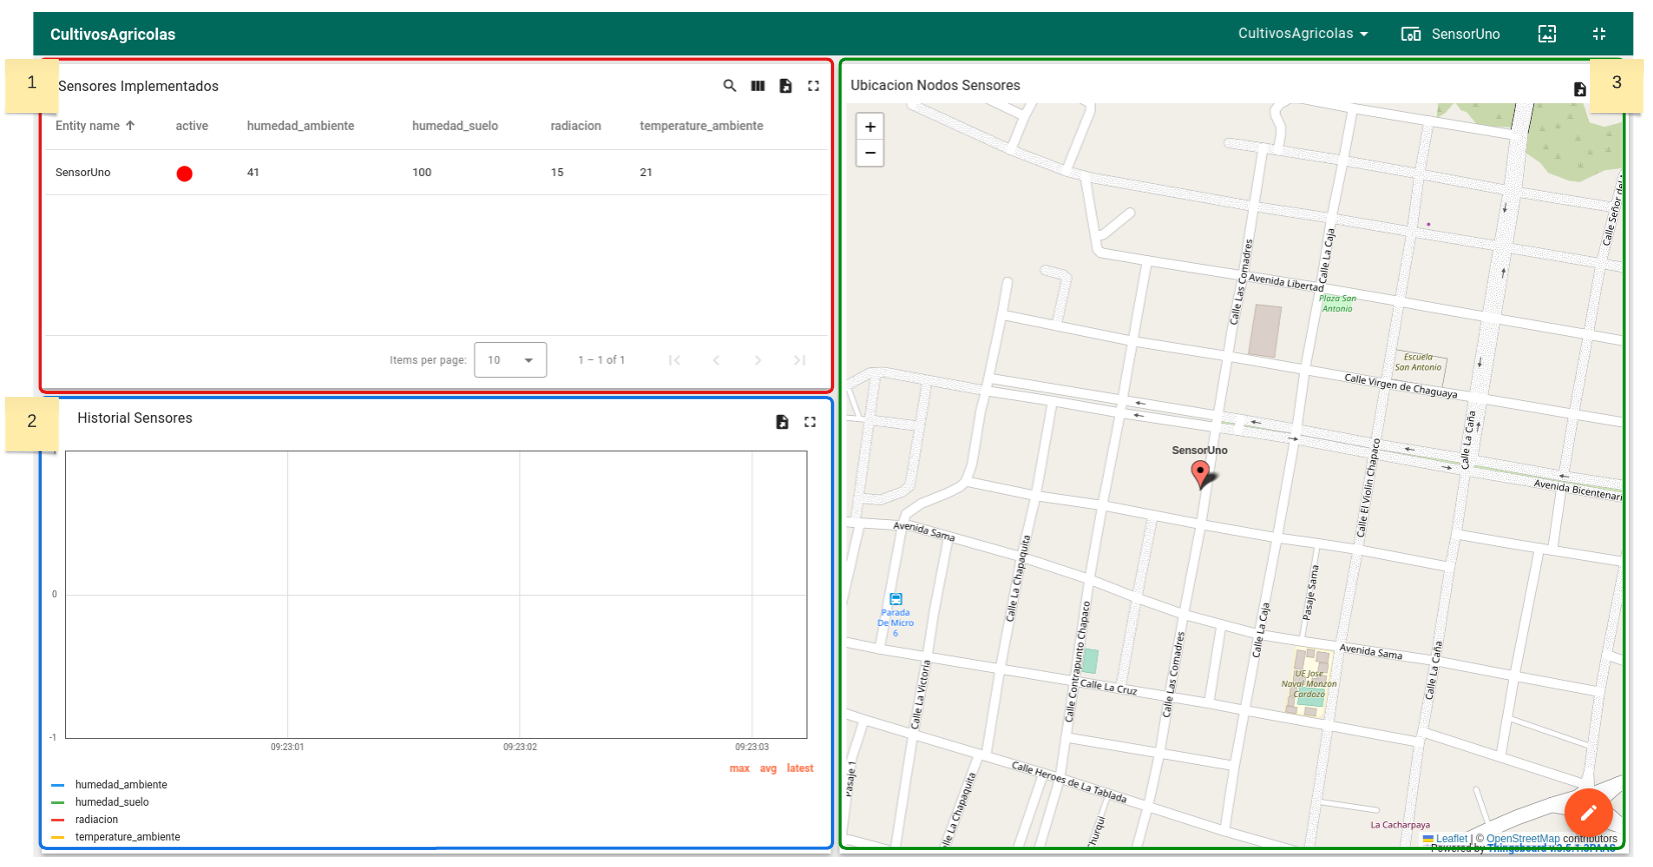
\includegraphics[width=\textwidth, height=8cm]{./Figures/panel_principal_editado.png}
  \caption{Panel principal de la interfaz gráfica.}
	\label{fig:Panel principal}
\end{figure}

\subsection{Panel nodo sensor} 

Para tener un mayor detalle de todos los parámetros de monitoreo de cada nodo sensor se creó un panel secundario que se muestra en la figura \ref{fig:Panel nodo sensor}.

El panel está dividido en las siguientes zonas:
\begin{itemize}
  \item Zona 1: gráficas que muestran los cambios que van teniendo los valores de las variables medidas por los sensores con respecto al tiempo.
  \item Zona 2: widgets que muestran el último valor obtenido por el nodo sensor de cada variable monitoreada.
  \item Zona 3: tabla que muestra las alarmas que se activaron. 
  \item Zona 4: se tiene un mapa que muestra la ubicación del nodo sensor implementado.
\end{itemize}

\begin{figure}[h!]
  \centering
	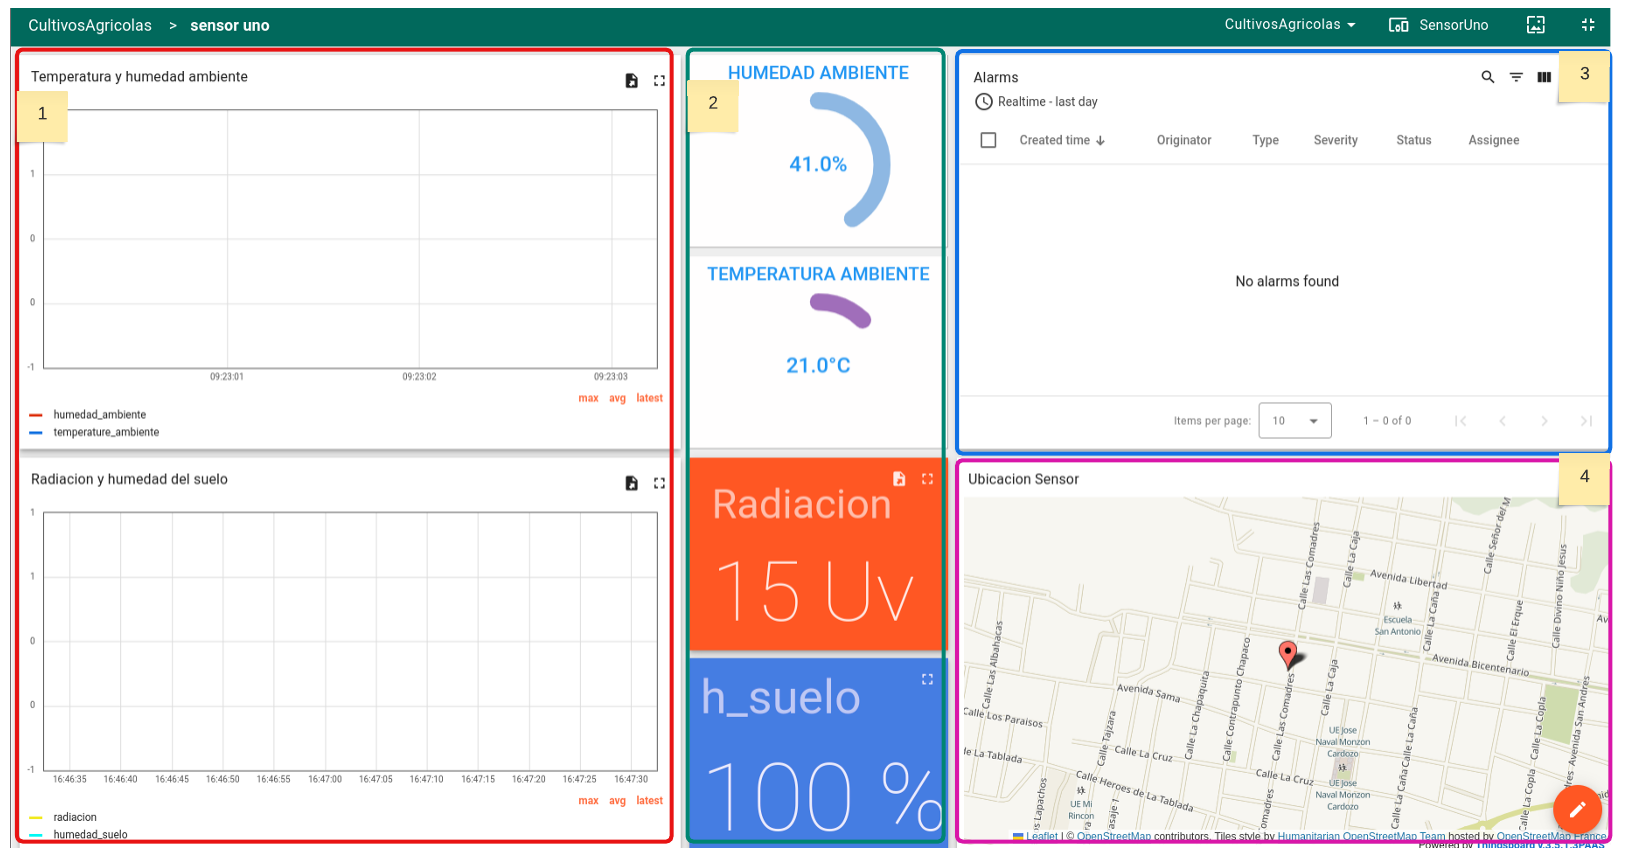
\includegraphics[width=\textwidth, height=8.5cm]{./Figures/panel_nodosensor_editado.png}
  \caption{Panel nodo sensor.}
	\label{fig:Panel nodo sensor}
\end{figure}
% Chapter Template

\chapter{Ensayos y resultados} % Main chapter title
En este capítulo se explican las pruebas realizadas al hardware, firmware, controladores y a la plataforma IoT.
\label{Chapter4} % Change X to a consecutive number; for referencing this chapter elsewhere, use \ref{ChapterX}

%----------------------------------------------------------------------------------------
%	SECTION 1
%----------------------------------------------------------------------------------------

\section{Pruebas unitarias}
Para la implementación de los drivers se utilizó la metodología de desarrollo TDD. Esto implica que se escribieron pruebas unitarias para los drivers. Se utilizó ceedling como herramienta de desarrollo de pruebas automáticas.

En el código \ref{cod:codigo test driver AHT10} se muestra la prueba implementada para la función de \emph{aht10\_get\_status()} del driver del sensor AHT10. Internamente utiliza funciones mock para la lectura y escritura por protocolo I2C, líneas 6,11 y 15. Se prueban dos casos: cuando la lectura de los registros es 0 y cuando es 255.
\begin{lstlisting}[label=cod:codigo test driver AHT10,caption=Tests del driver del sensor AHT10.]
//Prueba de funcion para obtener el estado del sensor AHT10
void test_estado_del_sensor(void)
{
  uint8_t buffer[1]={0};
  uint8_t data=0;
  read_I2C_STM32L432_port_ExpectAndReturn(AHT10_ADDRESS_SLAVE,buffer,1,AHT10_OK);
  read_I2C_STM32L432_port_ReturnThruPtr_buffer(&data);
  TEST_ASSERT_EQUAL(SENSOR_IDLE,aht10_get_status(&aht10config));
  
  data=255;
  read_I2C_STM32L432_port_ExpectAndReturn(AHT10_ADDRESS_SLAVE,buffer,1,AHT10_OK);
  read_I2C_STM32L432_port_ReturnThruPtr_buffer(&data);
  TEST_ASSERT_EQUAL(SENSOR_BUSY,aht10_get_status(&aht10config));
  
  read_I2C_STM32L432_port_ExpectAndReturn(AHT10_ADDRESS_SLAVE,buffer,1,AHT10_ERROR);
  TEST_ASSERT_EQUAL(SENSOR_BUSY,aht10_get_status(&aht10config)); 
}
\end{lstlisting}

En el código \ref{cod:codigo test driver bg96} se muestra la prueba desarrollada para la función \emph{send\_sms\_bg96()} encargada de mandar los mensajes de texto del driver BG96. Se probaron varios casos, cuando la función de envío de comandos responde con un OK y cuando responde con errores.
\begin{lstlisting}[label=cod:codigo test driver bg96,caption=Tests del driver del modulo bg96.] 
//Prueba de la funcion para mandar sms  
void test_send_sms_bg96(void)
{
  char buffer_resp[30]={0};
  send_data_ExpectAndReturn("AT+CMGS=\"72950576\"\r",RS_BG96_SIGNAL,buffer_resp,12000,FT_BG96_OK);
  send_data_ExpectAndReturn("HOLA\x1a\r",RS_BG96_OK,buffer_resp,12000,FT_BG96_OK);
  TEST_ASSERT_EQUAL(FT_BG96_OK,send_sms_bg96(&config_module,"72950576","HOLA"));

  send_data_ExpectAndReturn("AT+CMGS=\"72950576\"\r",RS_BG96_SIGNAL,buffer_resp,12000,FT_BG96_ERROR);
  TEST_ASSERT_EQUAL(FT_BG96_ERROR,send_sms_bg96(&config_module,"72950576","HOLA"));

  send_data_ExpectAndReturn("AT+CMGS=\"72950576\"\r",RS_BG96_SIGNAL,buffer_resp,12000,FT_BG96_OK);
  send_data_ExpectAndReturn("HOLA\x1a\r",RS_BG96_OK,buffer_resp,12000,FT_BG96_ERROR);
  TEST_ASSERT_EQUAL(FT_BG96_ERROR,send_sms_bg96(&config_module,"72950576","HOLA"));
}
\end{lstlisting}

Una forma cuantitativa de evaluar estas pruebas son los informes de cobertura generados por ceedling.

En la figura \ref{fig:Cobertura aht10} se puede observar el informe de cobertura del driver aht10, donde se puede apreciar que las pruebas ejecutan el 100\% de las líneas de código escritas y explora el 100\% de las combinaciones en los saltos de condicionales.

En la figura \ref{fig:Cobertura BG96} también se observa el informe de cobertura del driver de bg96, con 98.4\% de líneas ejecutadas y explora más del 98.3\% de combinaciones posibles. 

\begin{figure}[h!]
    \centering
      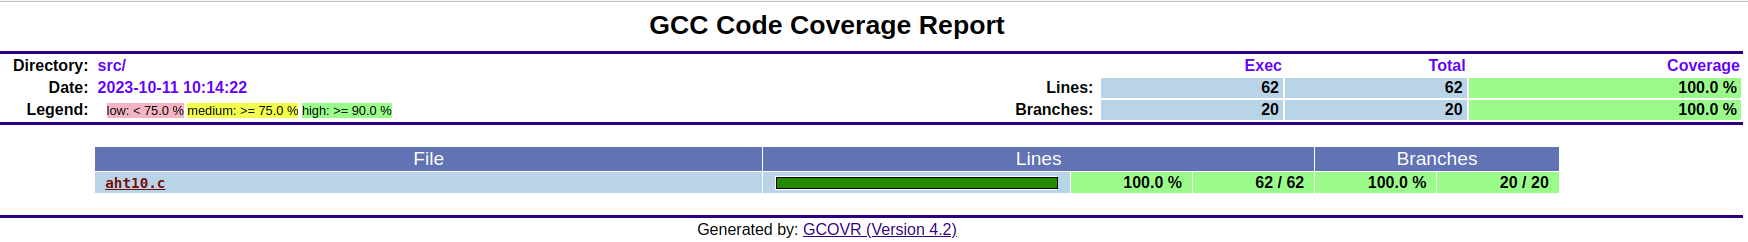
\includegraphics[width=\linewidth, height=4cm]{./Figures/cobertura_aht10.png}
    \caption{Informe de cobertura driver aht10.}
      \label{fig:Cobertura aht10}
  \end{figure}

\begin{figure}[h!]
    \centering
      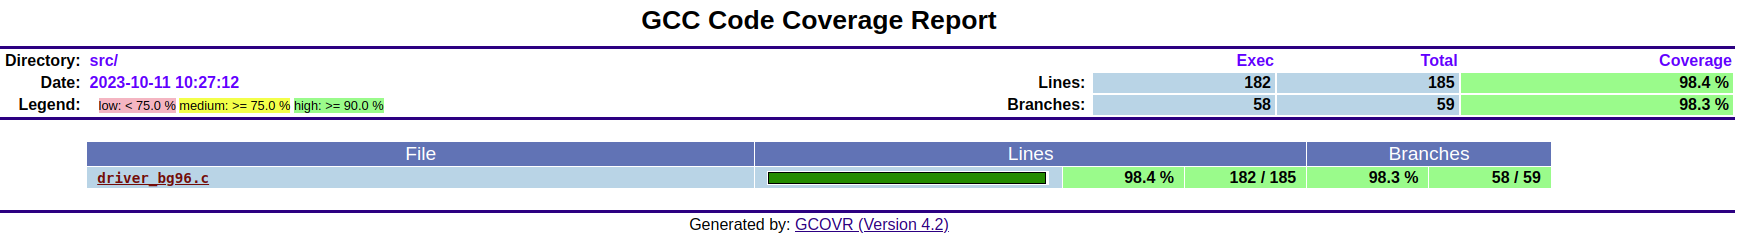
\includegraphics[width=\linewidth, height=4cm]{./Figures/cobertura_bg96.png}
    \caption{Informe de cobertura driver BG96.}
      \label{fig:Cobertura BG96}
\end{figure}

\section{Pruebas de la plataforma IoT}
\subsection{Prueba de inyección de mensajes}
El objetivo de la prueba de inyección de mensajes a la plataforma IoT, es verificar la llegada de los mensajes mandados por un cliente MQTT al broker de ThingsBoard.
Para realizar el envío de datos al broker, se utilizó el programa mosquitto. Para realizar esta prueba se ejecutó el comando de mosquitto que se muestra en la figura \ref{fig:mosquitto pub}.

\begin{figure}[h!]
  \centering
    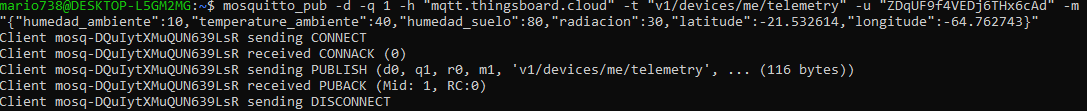
\includegraphics[width=\linewidth, height=3cm]{./Figures/mosquito_enviodatos.png}
  \caption{Envio de datos por el cliente MQTT de mosquitto.}
    \label{fig:mosquitto pub}
\end{figure}

Donde:
\begin{itemize}
  \item -h dirección del broker
  \item -t tópico 
  \item -u token
  \item -m mensaje en formato json
\end{itemize}

Al ejecutar el comando de la figura \ref{fig:mosquitto pub}, el cliente de mosquitto primeramente se conecta al broker MQTT, luego publica el mensaje en el tópico y finalmente, se desconecta del servidor.

Para comprobar la llegada de los datos al broker de ThingsBoard, se tiene que ir a la sección dispositivos, seleccionar el dispositivo al que se le envio los datos y entrar a la pestaña de última telemetría. En la figura \ref{fig:tb recepcion} podemos ver que los datos enviados llegan correctamente.

\begin{figure}[h!]
  \centering
    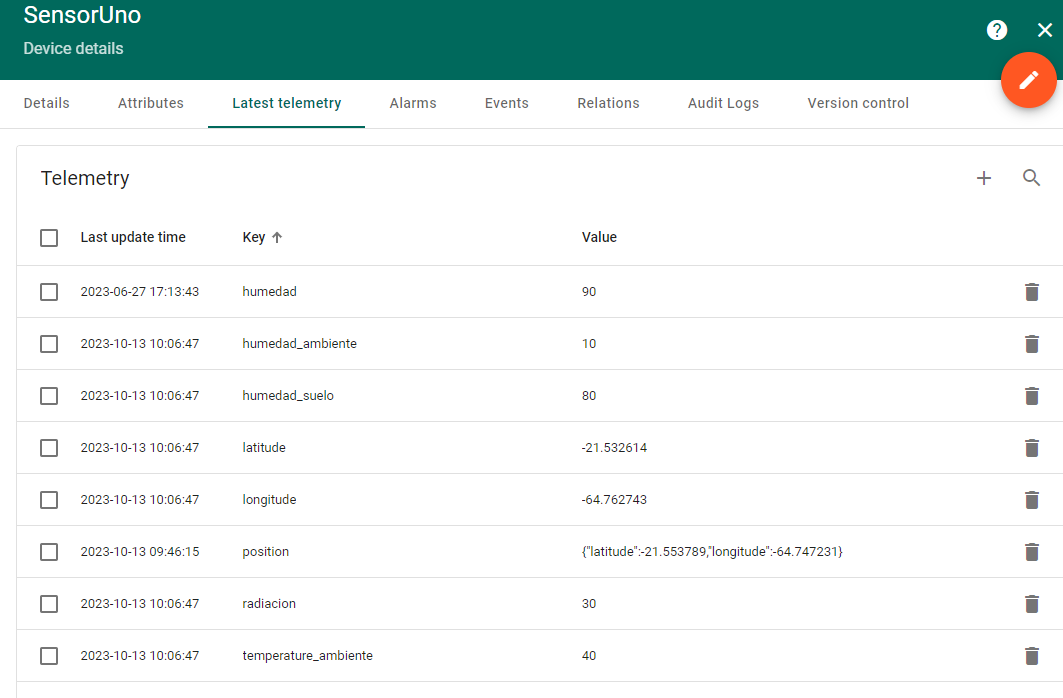
\includegraphics[width=5cm, height=6.5cm]{./Figures/tb_recepcion.png}
  \caption{Recepción de datos en el broker MQTT.}
    \label{fig:tb recepcion}
\end{figure}

\subsection{Prueba de la tabla de alarmas del panel visualización}
ThingsBoard permite configurar alarmas con respecto a las variables monitoreadas por el sistema. En el panel de visualización de cada sensor se tiene una tabla de alarmas, que muestra las notificaciones de las alarmas que se activaron.
En la figura \ref{fig:alarmas tb} podemos ver la notificación de una alarma cuando la temperatura ambiente sobrepasa los 43\textcelsius.

\begin{figure}[h!]
  \centering
    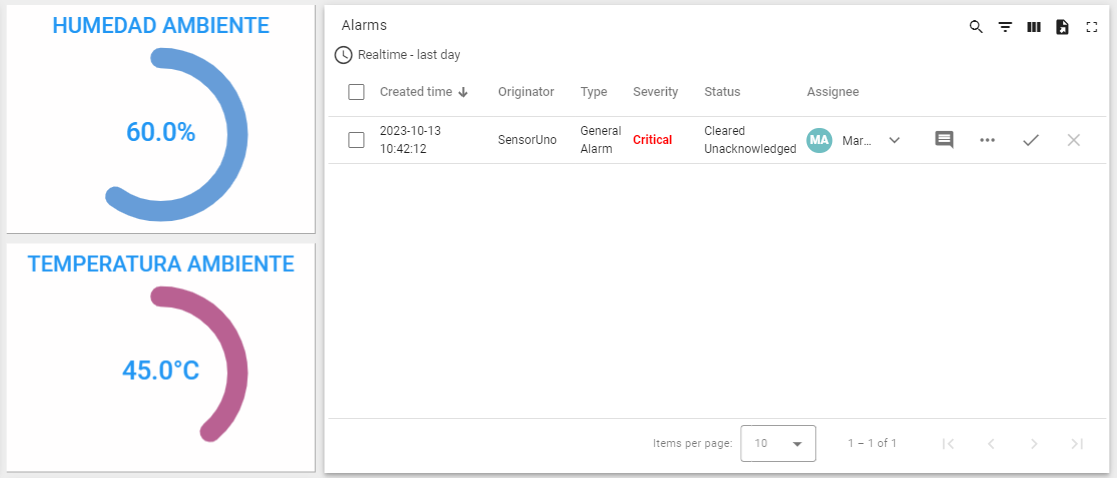
\includegraphics[width=\linewidth, height=7cm]{./Figures/alarmas_tb.png}
  \caption{Tabla de alarmas activas.}
    \label{fig:alarmas tb}
\end{figure}

\subsection{Prueba del widget de mapa}
En los paneles de visualización tenemos mapas que muestran la ubicación del dispositivo implementado.
En la figura \ref{fig:map thingsboard}  podemos ver la ubicación del prototipo implementado para el trabajo.

\begin{figure}[h!]
  \centering
    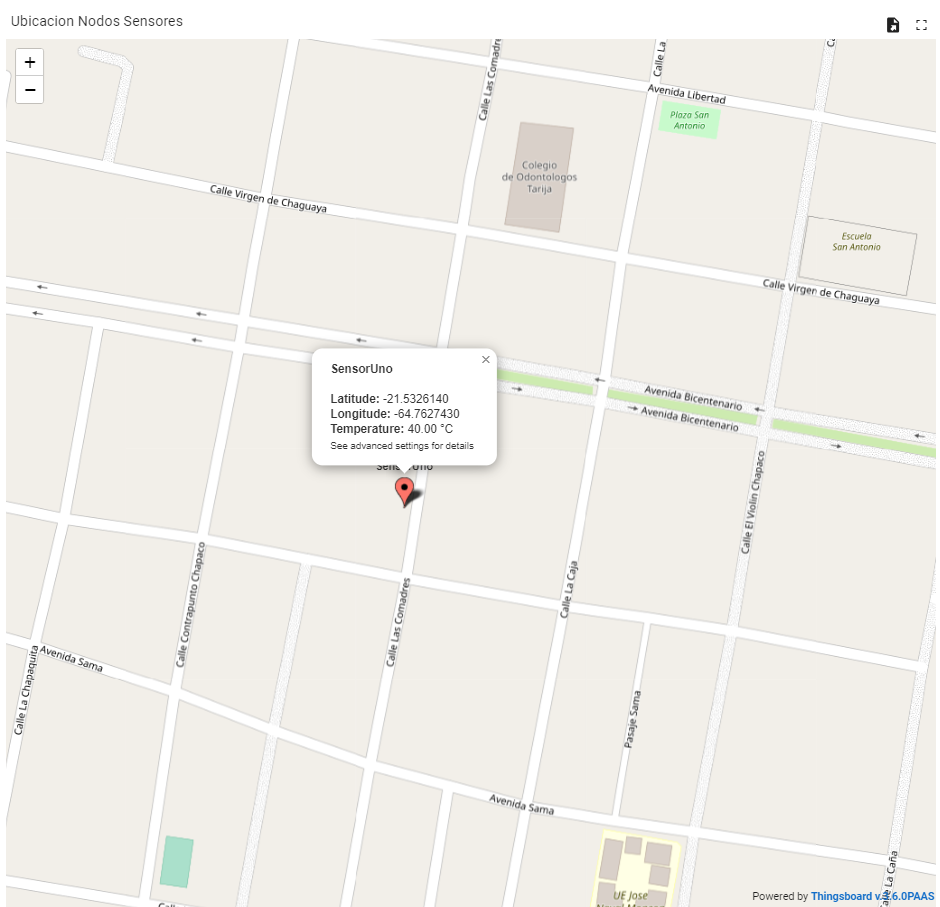
\includegraphics[width=10cm, height=6.5cm]{./Figures/map.png}
  \caption{Ubicación del nodo sensor implementado.}
    \label{fig:map thingsboard}
\end{figure}

\subsection{Prueba de persistencia de datos}
Para realizar la prueba de persistencia de datos, se configuró las gráficas de los paneles de visualización con un entorno de tiempo más amplio.
En las gráficas se estableció un rango de tiempo de 7 días. El resultado se muestra en la figura \ref{fig:Persistencia de datos}.

\begin{figure}[h!]
  \centering
    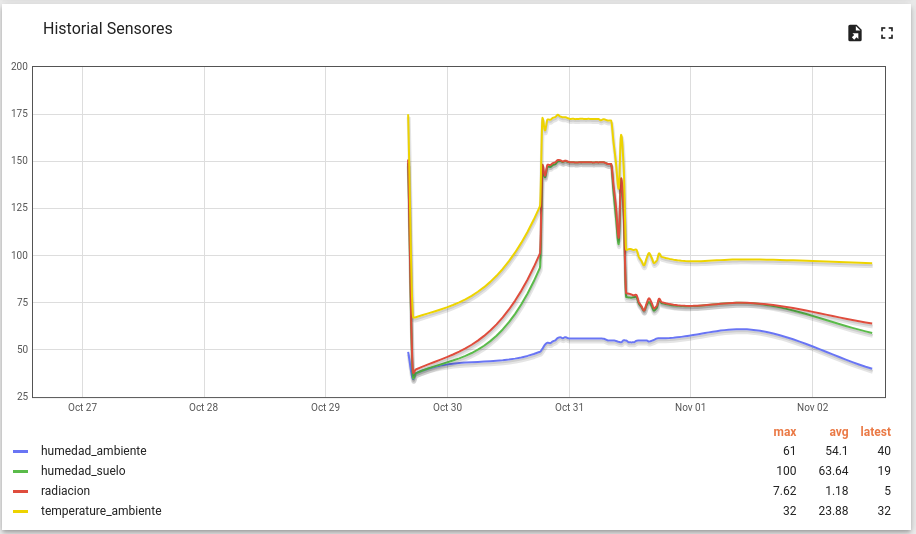
\includegraphics[width=10cm, height=6cm]{./Figures/persistencia_datos.png}
  \caption{Persistencia de datos.}
    \label{fig:Persistencia de datos}
\end{figure}

\section{Pruebas de hardware}
\subsection{Prueba de comunicación entre el sensor AHT10 y el microcontrolador}
Para comprobar la comunicación por I2C entre el sensor y el microcontrolador se utilizó un analizador lógico.
En la figura \ref{fig:write aht10} podemos ver la trama capturada por el analizador lógico cuando el firmware escribe en un registro del sensor. 

En la figura \ref{fig:read aht10} tenemos la trama capturada cuando se leen los registros del sensor. Se obtienen 6 bytes en los que se encuentra la información de la humedad y la temperatura.

\begin{figure}[h!]
  \centering
    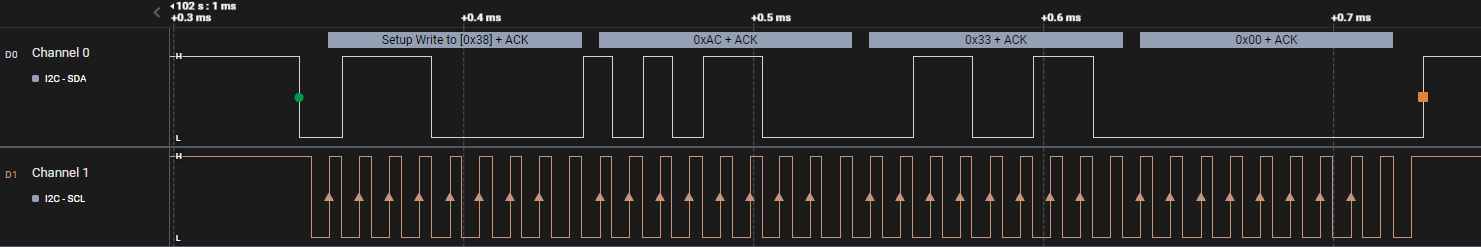
\includegraphics[width=\linewidth, height=3.2cm]{./Figures/write_i2c.png}
  \caption{Trama de escritura al sensor AHT10.}
    \label{fig:write aht10}
\end{figure}

\begin{figure}[h!]
  \centering
    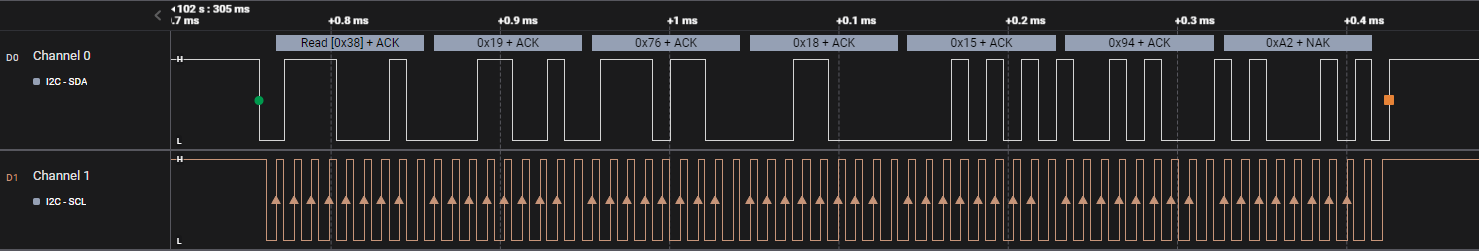
\includegraphics[width=\linewidth, height=3.5cm]{./Figures/read_i2c..png}
  \caption{Trama de lectura del sensor AHT10.}
    \label{fig:read aht10}
\end{figure}

\subsection{Prueba de comunicación entre el módulo BG96 y el microcontrolador}

Para probar la comunicación del microcontrolador con el módulo bg96, se utilizó un analizador lógico, que nos permite ver los comandos que envía el microcontrolador y la respuestas del módulo a estos comandos por protocolo serial.
En la figura \ref{fig:trama uart1} vemos dos canales del analizador  lógico: el canal 2 muestra un comando mandado por el microcontrolador al módulo de comunicación y en el canal 3 la respuesta del módulo al comando enviado.

\begin{figure}[h!]
  \centering
    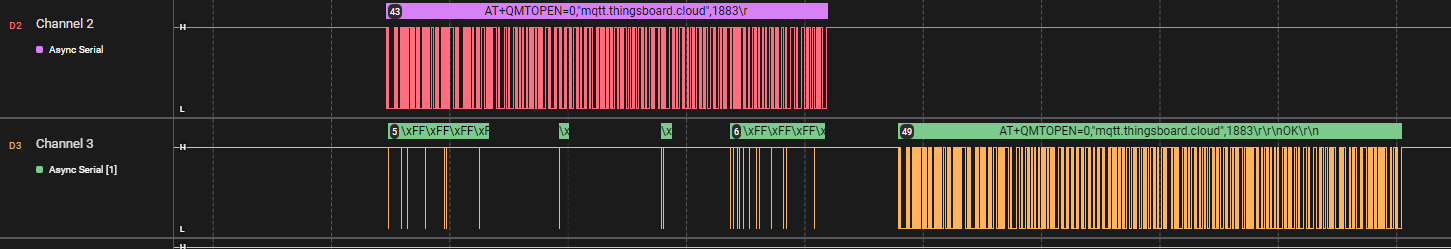
\includegraphics[width=\linewidth, height=3.5cm]{./Figures/trama_uart1.png}
  \caption{Envío y recepción de comandos por puerto UART.}
    \label{fig:trama uart1}
\end{figure}

\section{Pruebas funcionales del sistema}
Para realizar las pruebas funcionales de todo el sistema, se implementó el prototipo en un cultivo agrícola como se muestra en la figura \ref{fig:Condicionales ambientales prueba 1}.
\begin{figure}[h!]
  \centering
    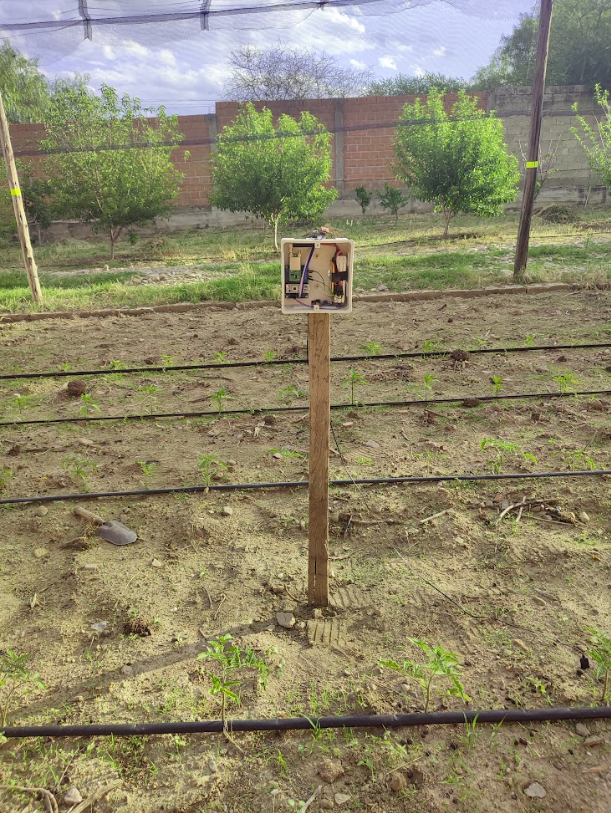
\includegraphics[width=5cm, height=5cm]{./Figures/prototipo_implementacion.png}
  \caption{Implementación del prototipo.}
    \label{fig:Condicionales ambientales prueba 1}
\end{figure}
  
\subsection{Pruebas de lectura de los sensores}
Se realizaron varias pruebas al prototipo en diferentes escenarios a continuación se desarrollaran algunas de las pruebas realizadas.
\subsubsection{Prueba uno}
La prueba consistió en realizar la lectura de los sensores en un momento donde se tenían las siguientes condiciones:
\begin{itemize}
  \item Tierra con poca humedad
  \item Temperatura ambiente alta 
  \item Horario de la lectura: 3 p.m
\end{itemize}
En la figura \ref{fig:Lectura tierra seca tb} se muestran los resultados de la lectura de los sensores en las condiciones anteriormente mencionadas. Se tiene una lectura de humedad de suelo de 19\%, radiación moderada de 5 y temperatura ambiente del 32\textcelsius.

\begin{figure}[h!]
  \centering
    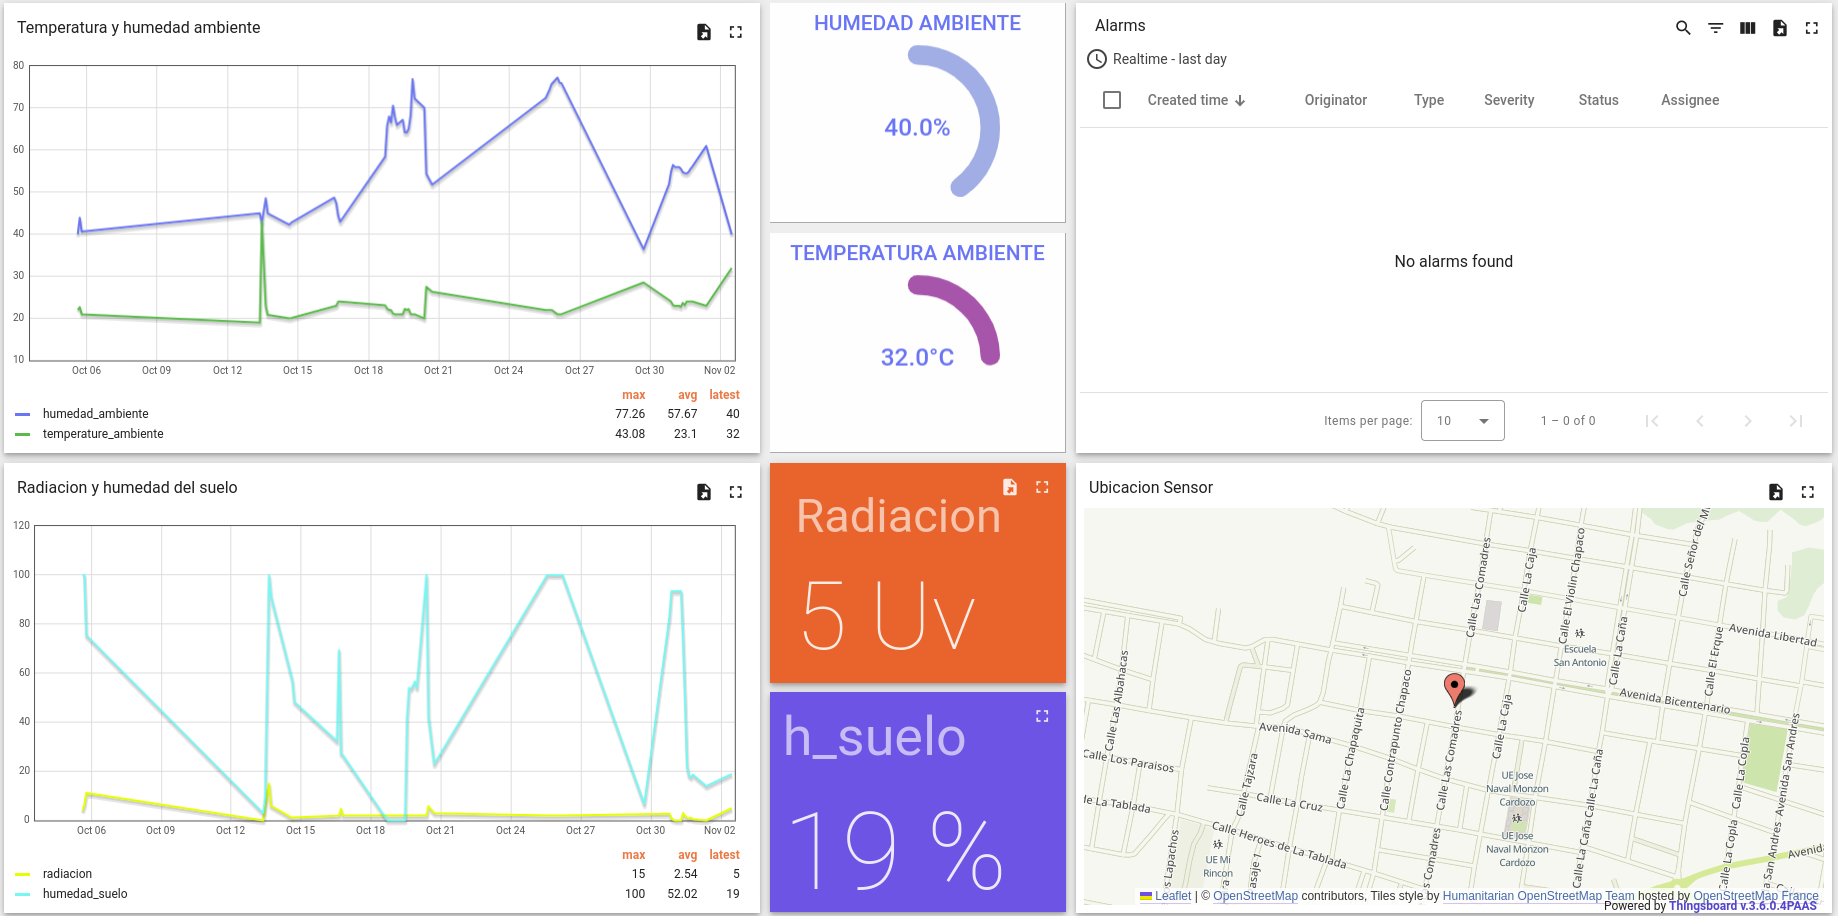
\includegraphics[width=\linewidth, height=6.5cm]{./Figures/tb_prueba1.png}
  \caption{Panel de visualización con las lecturas obtenidas en la prueba 1.}
    \label{fig:Lectura tierra seca tb}
\end{figure}

\subsubsection{Prueba dos}
Para la prueba dos se tenian las siguiente condiciones:
\begin{itemize}
  \item Tierra con humedad
  \item Temperatura moderada
  \item Horario de la lectura: 8 a.m
\end{itemize}

En la figura \ref{fig:Humedad alta ThingsBoard} se muestran los resultado de la lectura. Como resultado tenemos: humedad del suelo del 75\%, nivel de radiación baja de 2, humedad ambiente de 54\% y temperatura ambiente de 23\textcelsius.

\begin{figure}[h!]
  \centering
    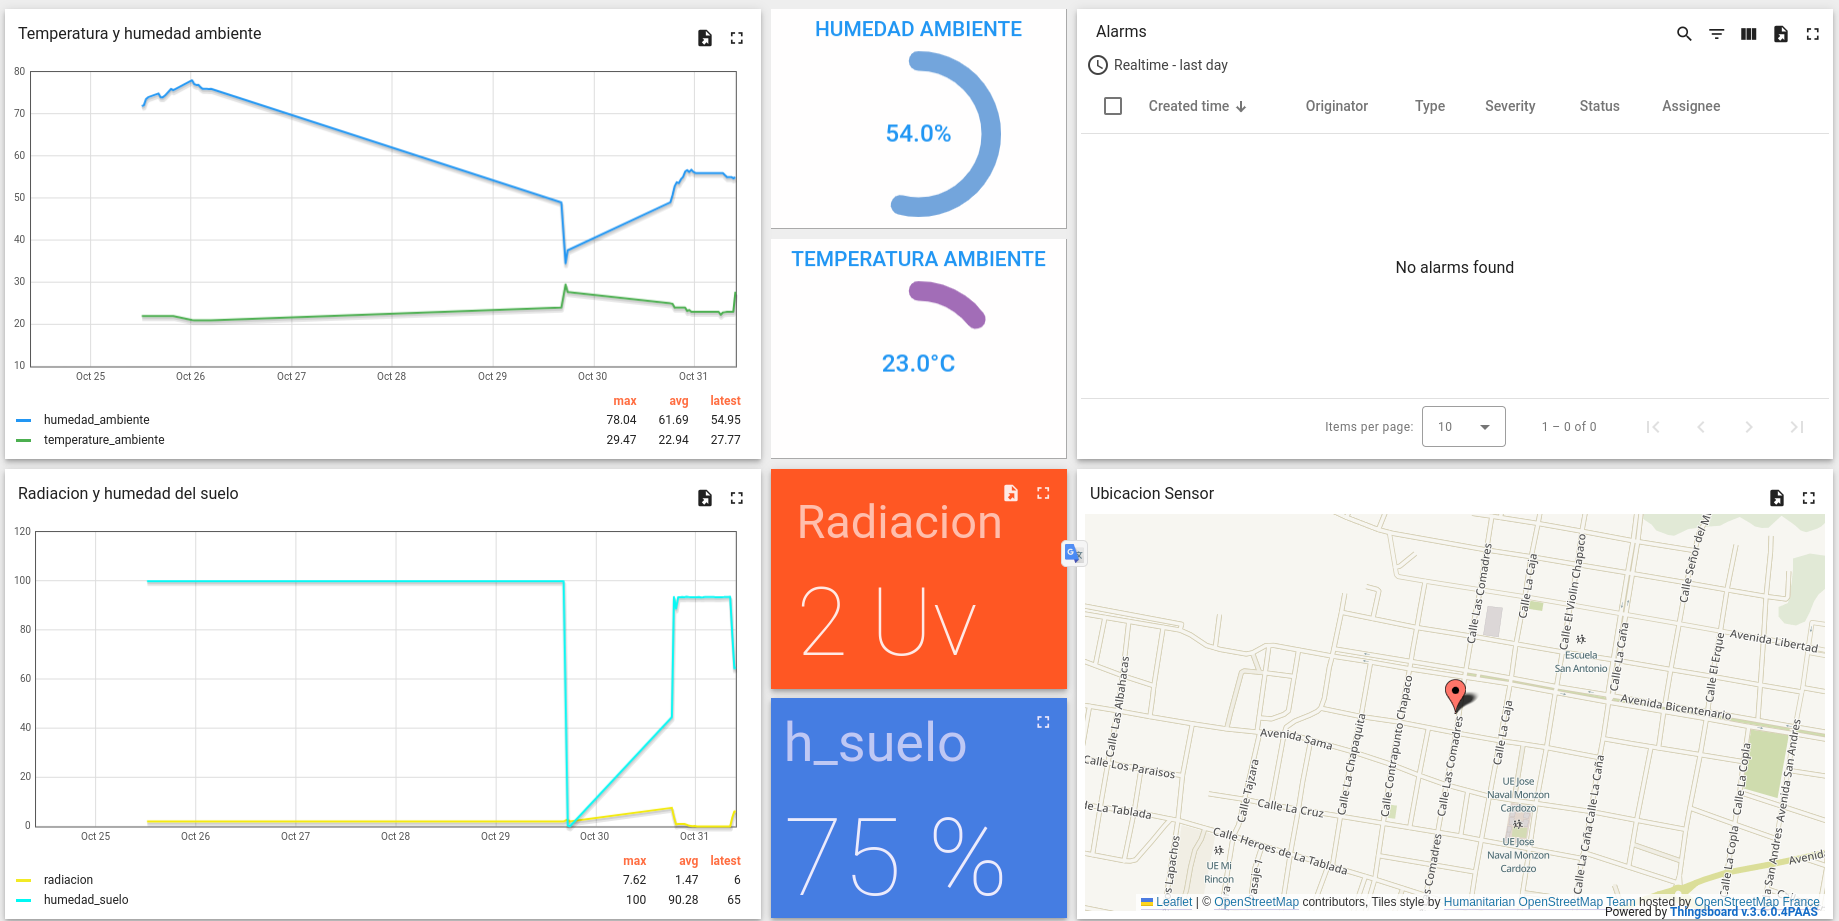
\includegraphics[width=\linewidth, height=6.5cm]{./Figures/humedad_alta_tb.png}
  \caption{Panel de visualización con las lecturas obtenidas en la prueba 2.}
    \label{fig:Humedad alta ThingsBoard}
\end{figure}

\subsection{Prueba del envío de datos al broker MQTT}
Una de las tareas más importante del firmware, es la del manejo de la comunicación con el servidor. Para verificar el funcionamiento de esta tarea, tenemos que ver la secuencia de comandos que manda el microcontrolador al módulo de comunicación.
Para realizar esta prueba se conectó un convertidor UART a USB al conector de depuración que tiene nuestro dispositivo.
En la figura \ref{fig:secuencia de comandos shell} podemos observar toda la secuencia de comandos que realiza el firmware para realizar el envío de datos a la plataforma IoT. Primeramente se envía el comando que verifica si el módulo está activo, luego se configura el apn de la red, se conecta al broker MQTT, se publican los datos y finalmente, se realiza el proceso de desconexión del broker.

\begin{figure}[h]
  \centering
    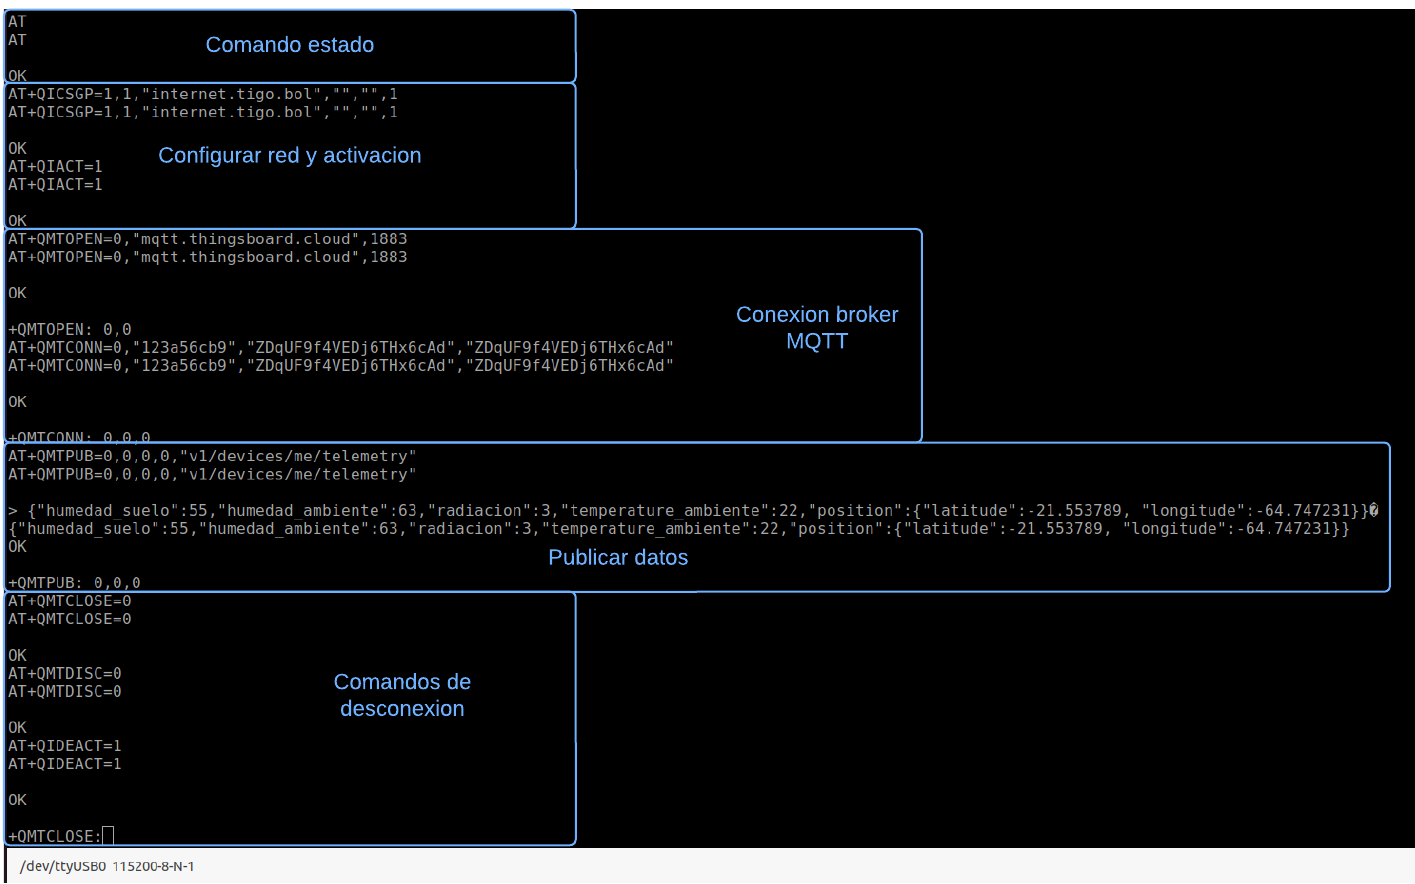
\includegraphics[width=12cm, height=9cm]{./Figures/secuencia de comandos shell.png}
  \caption{Comandos para enviar datos al broker MQTT.}
    \label{fig:secuencia de comandos shell}
\end{figure}

\subsection{Prueba de envio de alarmas por SMS}
El objetivo de esta prueba es verificar el funcionamiento de la alarma que monitorea la humedad del suelo.
Cuando la humedad del suelo baja por debajo del rango permitido. El firmware manda un SMS al usuario con el mensaje de "Humedad de suelo muy baja". En la figura \ref{fig:sms alarma} vemos que se recibió un SMS de alarma cuando la humedad bajó de 10\%.

\begin{figure}[h!]
  \centering
    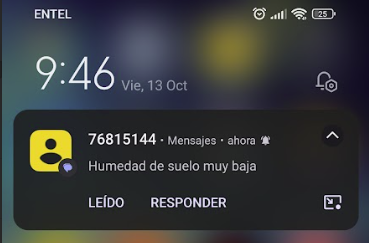
\includegraphics[width=5cm, height=3.5cm]{./Figures/sms_alarma2.png}
  \caption{Recepción del SMS con el mensaje  de alarma.}
    \label{fig:sms alarma}
\end{figure}

\label{sec:pruebasHW}

 
% Chapter Template

\chapter{Conclusiones} % Main chapter title
En este capítulo se presentan los resultados obtenidos sobre el trabajo realizado, las herramientas aprendidas durante el transcurso de la carrera que fueron fundamentales para la ejecución y se proponen ideas que permitan mejorar lo desarrollado.
\label{Chapter5} % Change X to a consecutive number; for referencing this chapter elsewhere, use \ref{ChapterX}

  
%----------------------------------------------------------------------------------------

%----------------------------------------------------------------------------------------
%	SECTION 1
%----------------------------------------------------------------------------------------

\section{Resultados obtenidos}
En el trabajo realizado se logró implementar de forma exitosa un prototipo correspondiente a un sistema de monitoreo de cultivos agrícolas. A través de las pruebas realizadas se pudo validar y demostrar su correcto funcionamiento.
Se pueden nombrar los siguientes logros obtenidos:
\begin{itemize}
\item Se fabricó un prototipo funcional y se lo instaló en un cultivo agrícola para la realización de pruebas integrales del sistema, garantizando cumplir todos los requerimientos funcionales.
\item Se diseñó el esquemático y el PCB de la tarjeta electrónica para el prototipo.
\item Se desarrolló el firmware sobre un sistema operativo de tiempo real, para optimizar los recursos del microcontrolador y hacer un código más modular y escalable.
\item Se configuraron paneles de visualización en ThingsBoard. Permitiendo visualizar las variables ambientales adquiridas por el prototipo instalado en el  cultivo agrícola.
\item Se implementó el envío de alarmas del sistema al usuario mediante SMS.
\item Se utilizó Git para control de versiones, ayudó a tener la trazabilidad y flexibilidad necesaria para llevar a cabo el desarrollo de manera ordenada.
\end{itemize}

Los requerimientos del trabajo fueron cubiertos de acuerdo con la planificación, con la siguiente modificación:

\begin{itemize}
    \item Se cambió el requerimiento de utilizar HTTP como protocolo de envío de datos a la nube. Se utilizó MQTT porque es un protocolo más rápido, liviano y utiliza el modelo publicador/suscriptor.
\end{itemize}

En el desarrollo del trabajo se aplicaron muchos de los conocimientos adquiridos a lo largo de la Carrera de Especialización en Sistemas Embebidos. Entre los conocimientos aplicados, se pueden destacar los adquiridos en las siguientes asignaturas:

\begin{itemize}
    \item Programación de Microcontroladores: se utilizaron conceptos básicos de programación, conceptos de modularización y uso de patrones de diseño. 
    \item Protocolos de Comunicación en Sistemas Embebidos: se utilizaron protocolos de comunicación I2C, UART y MQTT.
    \item Sistemas Operativos de Tiempo Real: se implementó el firmware sobre freeRTOS. Se utilizaron colas y semáforos, para la comunicación y sincronización entre tareas.    
    \item Testing de Software en Sistemas Embebidos: uso de TDD para el desarrollo de los drivers. Se utilizó Ceedling para el desarrollo de pruebas automáticas.
    \item Diseño de Circuitos Impresos: se utilizaron buenas prácticas de diseño electrónico para desarrollar el esquemático y el circuito impreso del prototipo. Se utilizó KICAD como herramienta de diseño electrónico.
\end{itemize}

%----------------------------------------------------------------------------------------
%	SECTION 2
%----------------------------------------------------------------------------------------
\section{Próximos pasos}

Si bien se lograron obtener los resultados esperados, a futuro se puede continuar
con el desarrollo en varias medidas. A continuación, se detallan los aspectos que sería conveniente tomar en consideración:
\begin{itemize}
    \item Realizar un nuevo diseño del hardware que integre a todo el sistema y no utilice módulos por separado.
    \item Implementar un mecanismo de actualización de firmware remoto.
    \item Incluir soporte para trabajar con energías renovables.
    \item Aumentar la seguridad al enviar los datos al servidor utilizando SSL.
\end{itemize} 

%----------------------------------------------------------------------------------------
%	CONTENIDO DE LA MEMORIA  - APÉNDICES
%----------------------------------------------------------------------------------------

\appendix % indicativo para indicarle a LaTeX los siguientes "capítulos" son apéndices

% Incluir los apéndices de la memoria como archivos separadas desde la carpeta Appendices
% Descomentar las líneas a medida que se escriben los apéndices

%% Appendix A

\chapter{Appendix Title Here} % Main appendix title

\label{AppendixA} % For referencing this appendix elsewhere, use \ref{AppendixA}

Write your Appendix content here.
%\include{Appendices/AppendixB}
%\include{Appendices/AppendixC}

%----------------------------------------------------------------------------------------
%	BIBLIOGRAPHY
%----------------------------------------------------------------------------------------

\Urlmuskip=0mu plus 1mu\relax
\raggedright
\printbibliography[heading=bibintoc]

%----------------------------------------------------------------------------------------

\end{document}  
